\documentclass{article}
\usepackage[utf8]{inputenc}
\usepackage{array}
\usepackage{multirow}
\usepackage{graphicx}
\usepackage{color}   %May be necessary if you want to color links
\usepackage{hyperref}
\usepackage{longtable}
\usepackage{float}
\usepackage[table]{xcolor}
\usepackage{amssymb}
\usepackage{minted}
\usepackage{rotating}
\setlength{\arrayrulewidth}{0.5mm}
\setlength{\tabcolsep}{18pt}
\renewcommand{\arraystretch}{2.5}
\hypersetup{
    colorlinks=false, %set true if you want colored links
    linktoc=all,     %set to all if you want both sections and subsections linked
    %linkcolor=blue,  %choose some color if you want links to stand out
}

\title{DREAM - DD}
\author{Filippo Lazzati}
%\date{October 2021}

\begin{document}
\thispagestyle{empty} 
\begin{titlepage}
    \begin{center}
       %\vspace*{2cm}
       {\Huge \textbf{DREAM}} %%Replace this with the Title of your research
       \vspace{0.5cm}
       \\
    \begin{LARGE}
        {Data-dRiven PrEdictive FArMing in Telangana}
        \vspace{1.0cm}
        \\
        {\textit{Design Document - DD}}
        
\includegraphics[width=13cm]{logo/polimi.png}
       \vspace{1.5cm}
        
        {Christian Grasso - Filippo Lazzati - Chiara Magri}
       \vspace{0.5cm}
       {Year: 2021/2022}
       
    \end{LARGE}  
   \end{center}
\end{titlepage}
\newpage
\tableofcontents %this command creates an index
\newpage

\section{Introduction}
A DD\footnote{Design Document. See section \ref{Abbreviations}}, according to the definition provided by the \textbf{IEEE Std 1016™-2009} standard, is \textit{a representation of a software design that is to be used for recording design information, addressing various design concerns, and communicating that information to the design’s stakeholders}. It should be noticed that, in this document, instead of using the abbreviation SDD, which stands for "Software Design Description", is used DD. In other words, a DD is a document that is used by \textit{acquirers, project managers, quality assurance staff, configuration managers, software designers, programmers, testers, and maintainers} to retrieve the specific design information needed by the specific stakeholder.
\subsection{Purpose}\label{Purpose}
\verb|DREAM|, the system to-be, aims to help policy makers 
formulating policies in the field of agriculture.  Moreover, \verb|DREAM| aims to help farmers by putting them in contact with each other so that they can exchange advice and aids. Finally, \verb|DREAM| also schedules the daily work of agronomists and make them visit the worse-performing farmers. These are the main goals of \verb|DREAM| which shall be data-driven, namely it shall intensively exploits data to perform the tasks it is asked to do. The requirements that allow the system to satisfy the goals as well as a detailed list of all the goals are present respectively in \textit{RASD - 3.2 Functional requirements} and in \textit{RASD - 1.1 Purpose}. In this document the focus in on the design, that is on the description of the components and the interaction among them and with external systems through interfaces which compose the system and allow the satisfaction of the requirements and, at the end, of the goals.
\subsection{Scope}
The system to-be has three major stakeholders: the policy makers, the agronomists and the farmers. The needs that \verb|DREAM| aims to satisfy differ among them, and the main goals of the system have been identified in section\ref{Purpose}. For a detailed description and explanation of the context in which \verb|DREAM| operates the reader should refer to the \textit{RASD - 1.2 Scope} section. In here, we briefly tell about the main design concerns of such stakeholders.\\
First of all, all of them have goals that, in order to be satisfied, require the storage of a large volume of data (after all, \verb|DREAM| is a data-driven system), and therefore scalable technologies suitable to manage the required amount of information have to be used. Furthermore, the stakeholders are not assumed to be expert in computer science, thus a graphical interface is needed; more specifically, the idea is to implement a web application to facilitate the access to the system to all the users and from any kind of device (computer, smartphone, ...).
\subsection{Definitions, Acronyms, Abbreviations}\label{Abbreviations}
This section provides a list of the main abbreviations, acronyms and definitions adopted in the document:
\begin{itemize}
    \item Design Document (DD): "An SDD is a representation of a software design to be used for communicating design information to its stakeholders. The requirements for the design languages (notations and other representational schemes) to be used for conformant SDDs are specified.
    \item RASD
    \item IFML
    \item UI
This standard is applicable to automated databases and design description languages but can be
used for paper documents and other means of descriptions".
\end{itemize}
\subsection{Revision history}
\raggedright
\begin{tabular}{ |c | c |}
\hline
 \textit{revision} & \textit{changes} \\ 
 \hline
 1.0 &  initial version\\ 
 \hline
\end{tabular}
\subsection{Reference Documents}
\begin{itemize}
    \item \textit{IEEE Std 1016™-2009}, the standard for information technology, systems design, Software Design Descriptions. It describes the "required information content and organization for software design descriptions (SDDs)";
    \item \textit{ISO/IEC/IEEE 42010}, the standard for architecture description in systems and software engineering, that "addresses the creation, analysis and sustainment of architectures of systems
through the use of architecture descriptions".
\end{itemize}
\subsection{Document Structure}
This document complies with the SDD\footnote{Software Design Descriptions} standard structure as it is defined in the \textit{IEEE Std 1016™-2009}, sections 4 and 5. Nevertheless, the contents have been ordered in a way that best fits the specific topics of this document and to facilitate the readers in the reading of this DD\footnote{Design Document.}.
The document is divided in 5 main parts:
\begin{enumerate}
\item the first part (to which this section belongs) provides an introduction to the system to-be, \verb|DREAM|, helping in the reading of the following sections;
\item the second part provides the out-and-out design decisions under which \verb|DREAM| is implemented. This part contains UML\footnote{Unified Modeling Language.} diagrams as well as text descriptions of the components of the system along with their interfaces, and explanations of the selected architectural styles and design patterns and possible other design decisions;
\item the third part describes the user interface. This part is a continuation of the \textit{RASD - 3.1.1 User Interfaces} section, which enters the details of the design choices;
\item the fourth part shows how the requirements identified in the \textit{RASD - 3.2 Functional requirements} section have brought to the introduction of a specific component/interface in the system;
\item the fifth and last part is about a plan to follow for the implementation of the system, namely from which subcomponent to start, which subcomponents can be implemented in parallel, and about a plan for the integration of such subcomponents and also a plan for testing the integration.
\end{enumerate}
It should be remarked that the structure of this document does not follow a logic or temporal order, but whoever is interested in the reading can jump from a section to another, because the purpose of it is to be a reference document.\newpage
\section{Architectural design}
\subsection{Overview}
In this section, an high-level overview of the design components is provided.\\
The architecture chosen is a three-tier one, in which there is a clear-cut separation between the three tiers. The reasons behind this choice comprise mainly the scalability, the accessibility and the security of this solution; they are explained more in detail in section \ref{Architectural style}.
An high-level view of the entire architecture of \verb|DREAM| is illustrated in figure \ref{fig:overview}:
\begin{figure}[H]
    \centering
    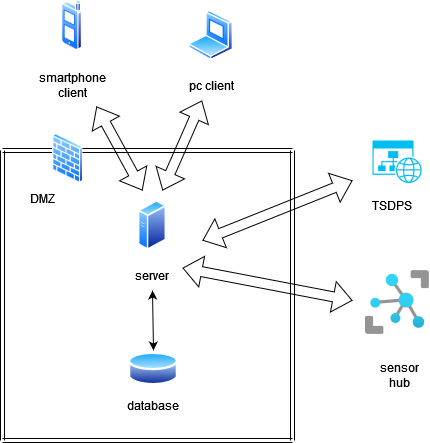
\includegraphics[scale=0.5]{diagrams/overview.png}
    \caption{The main high-level components of the system.}
    \label{fig:overview}
\end{figure}
As previously said, the system has a three-tier architecture\footnote{Notice that it is not always true that logical layers (presentation, application and data) are mapped 1-to-1 to physical layers (tiers). As far as DREAM is concerned, this is true.}.
\paragraph{Tier 1 - Presentation layer}
The first tier is composed of a webapp installed on the device of the user; the device of the user can be any, as long as it has a browser installed and can be connected to Internet (in the figure this fact is exemplified through a smartphone and a pc). This is the tier closest to the user, and its role is basically related to managing the interaction with the user. It is the actual frontend, and in \verb|DREAM| it is provided with a GUI (Graphical User Interface). It should be remarked that the logic of the system is not present here, but is contained in the application layer.
\paragraph{Tier 2 - Application layer}
The second tier of the application has the fundamental role of managing all the functions that are available to the user. Here lies the business logic of \verb|DREAM|, which interacts with the other two tiers and with external services to perform all the activities of the system. This layer is exemplified by the high-level server component in figure \ref{fig:overview}. As it is explained in the following section, such layer is made of various \textit{services}, each of them associated to a specific function.
\paragraph{Tier 3 - Data layer}
The third tier is exemplified with a database and contains all the data \verb|DREAM| has to store. As a matter of fact, \verb|DREAM| is a data-driven application, and as such has to cope with a large amount of data to carry out its activities. All this data is stored in a database, which can be accessed by the application layer through a particular interface, as can be noticed in the following section. Along with the second tier, the third tier represents the backend of the system, which is protected inside a demilitarized zone\footnote{A DMZ is a subnetwork that contains and exposes important services and data of a company to an untrusted network (Internet in this case); the main goal is higher protection.} (DMZ).
\paragraph{External services}
TSDP (external weather service) and the sensor hub are two external high-level components \verb|DREAM| has to interact with. The former provides weather reports and forecasts, while the latter allows \verb|DREAM| to access sensors and water irrigation system data. 
\subsection{Component view}\label{Component view}
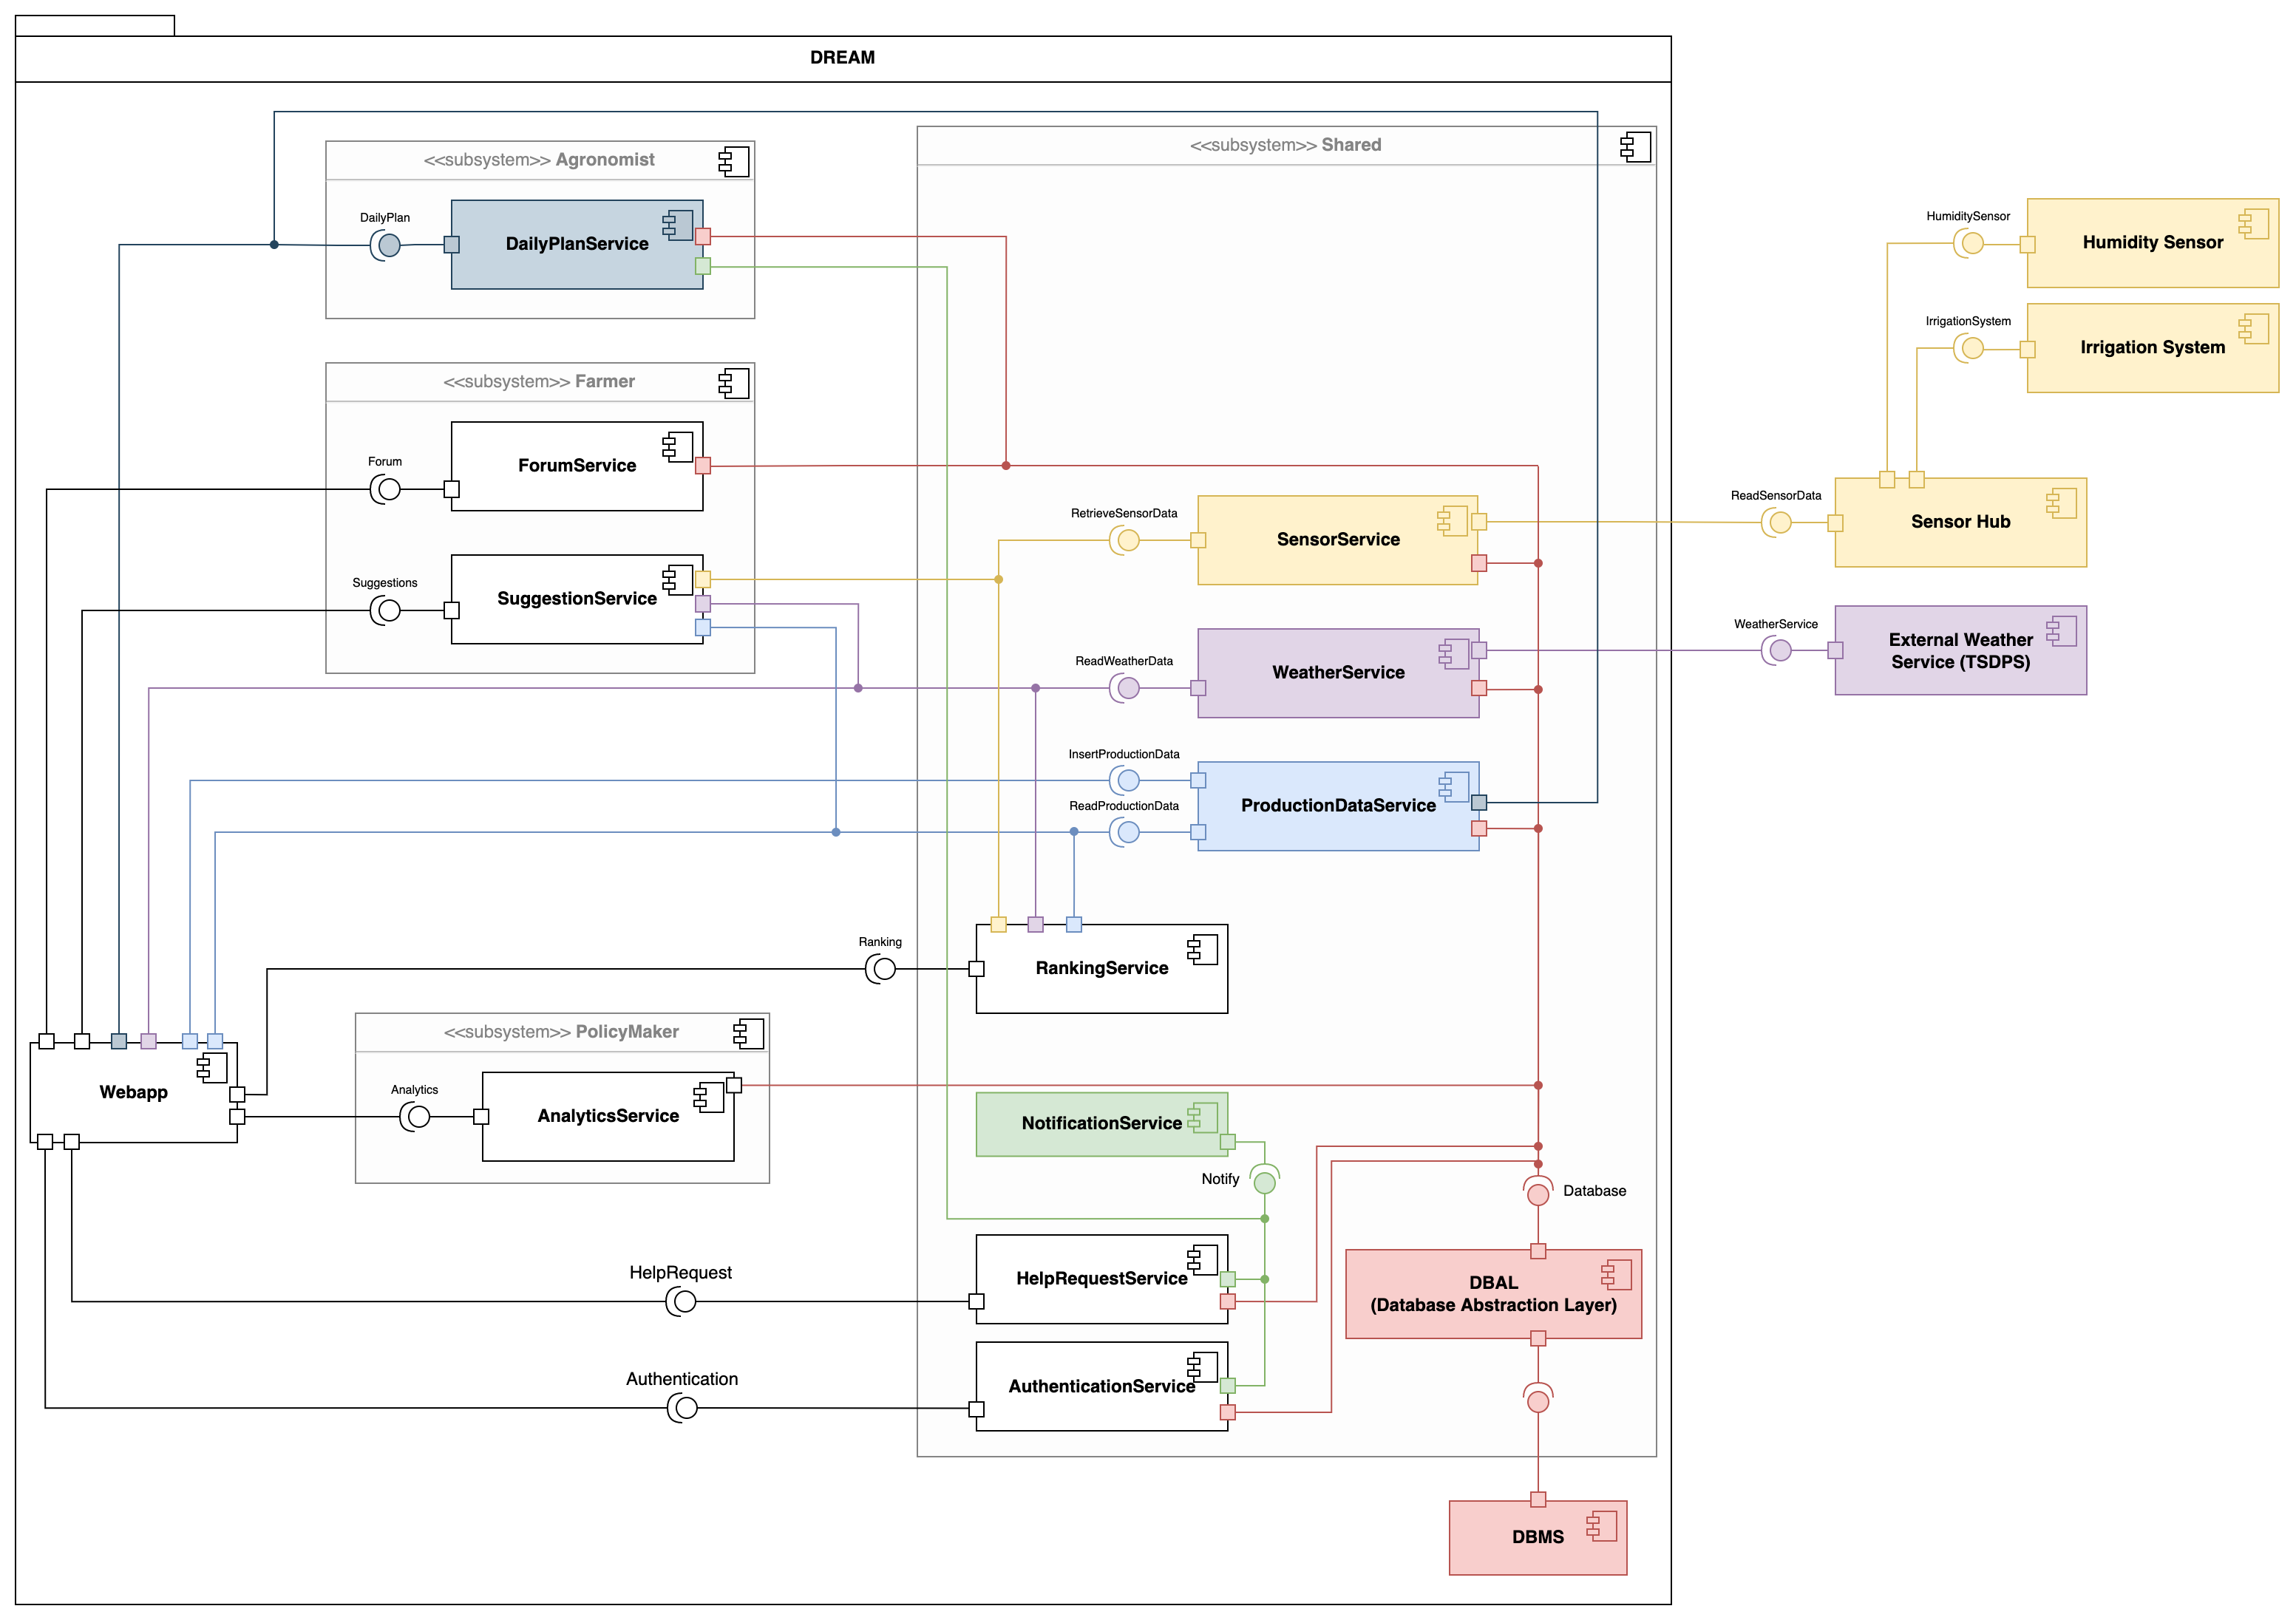
\includegraphics[width=16.5cm]{diagrams/components_diagram.png}
\subsection{Deployment view}
By the definition provided in "The Unified Modeling Language User Guide"\footnote{ISBN: 0-201-57168-4}, a deployment diagram is \textit{a diagram that shows the configuration of run time processing nodes and the components that live on them}. In other words, we represent the topology of processors and devices where our software executes.\\
The deployment diagram of \verb|DREAM| is the following:
\newpage
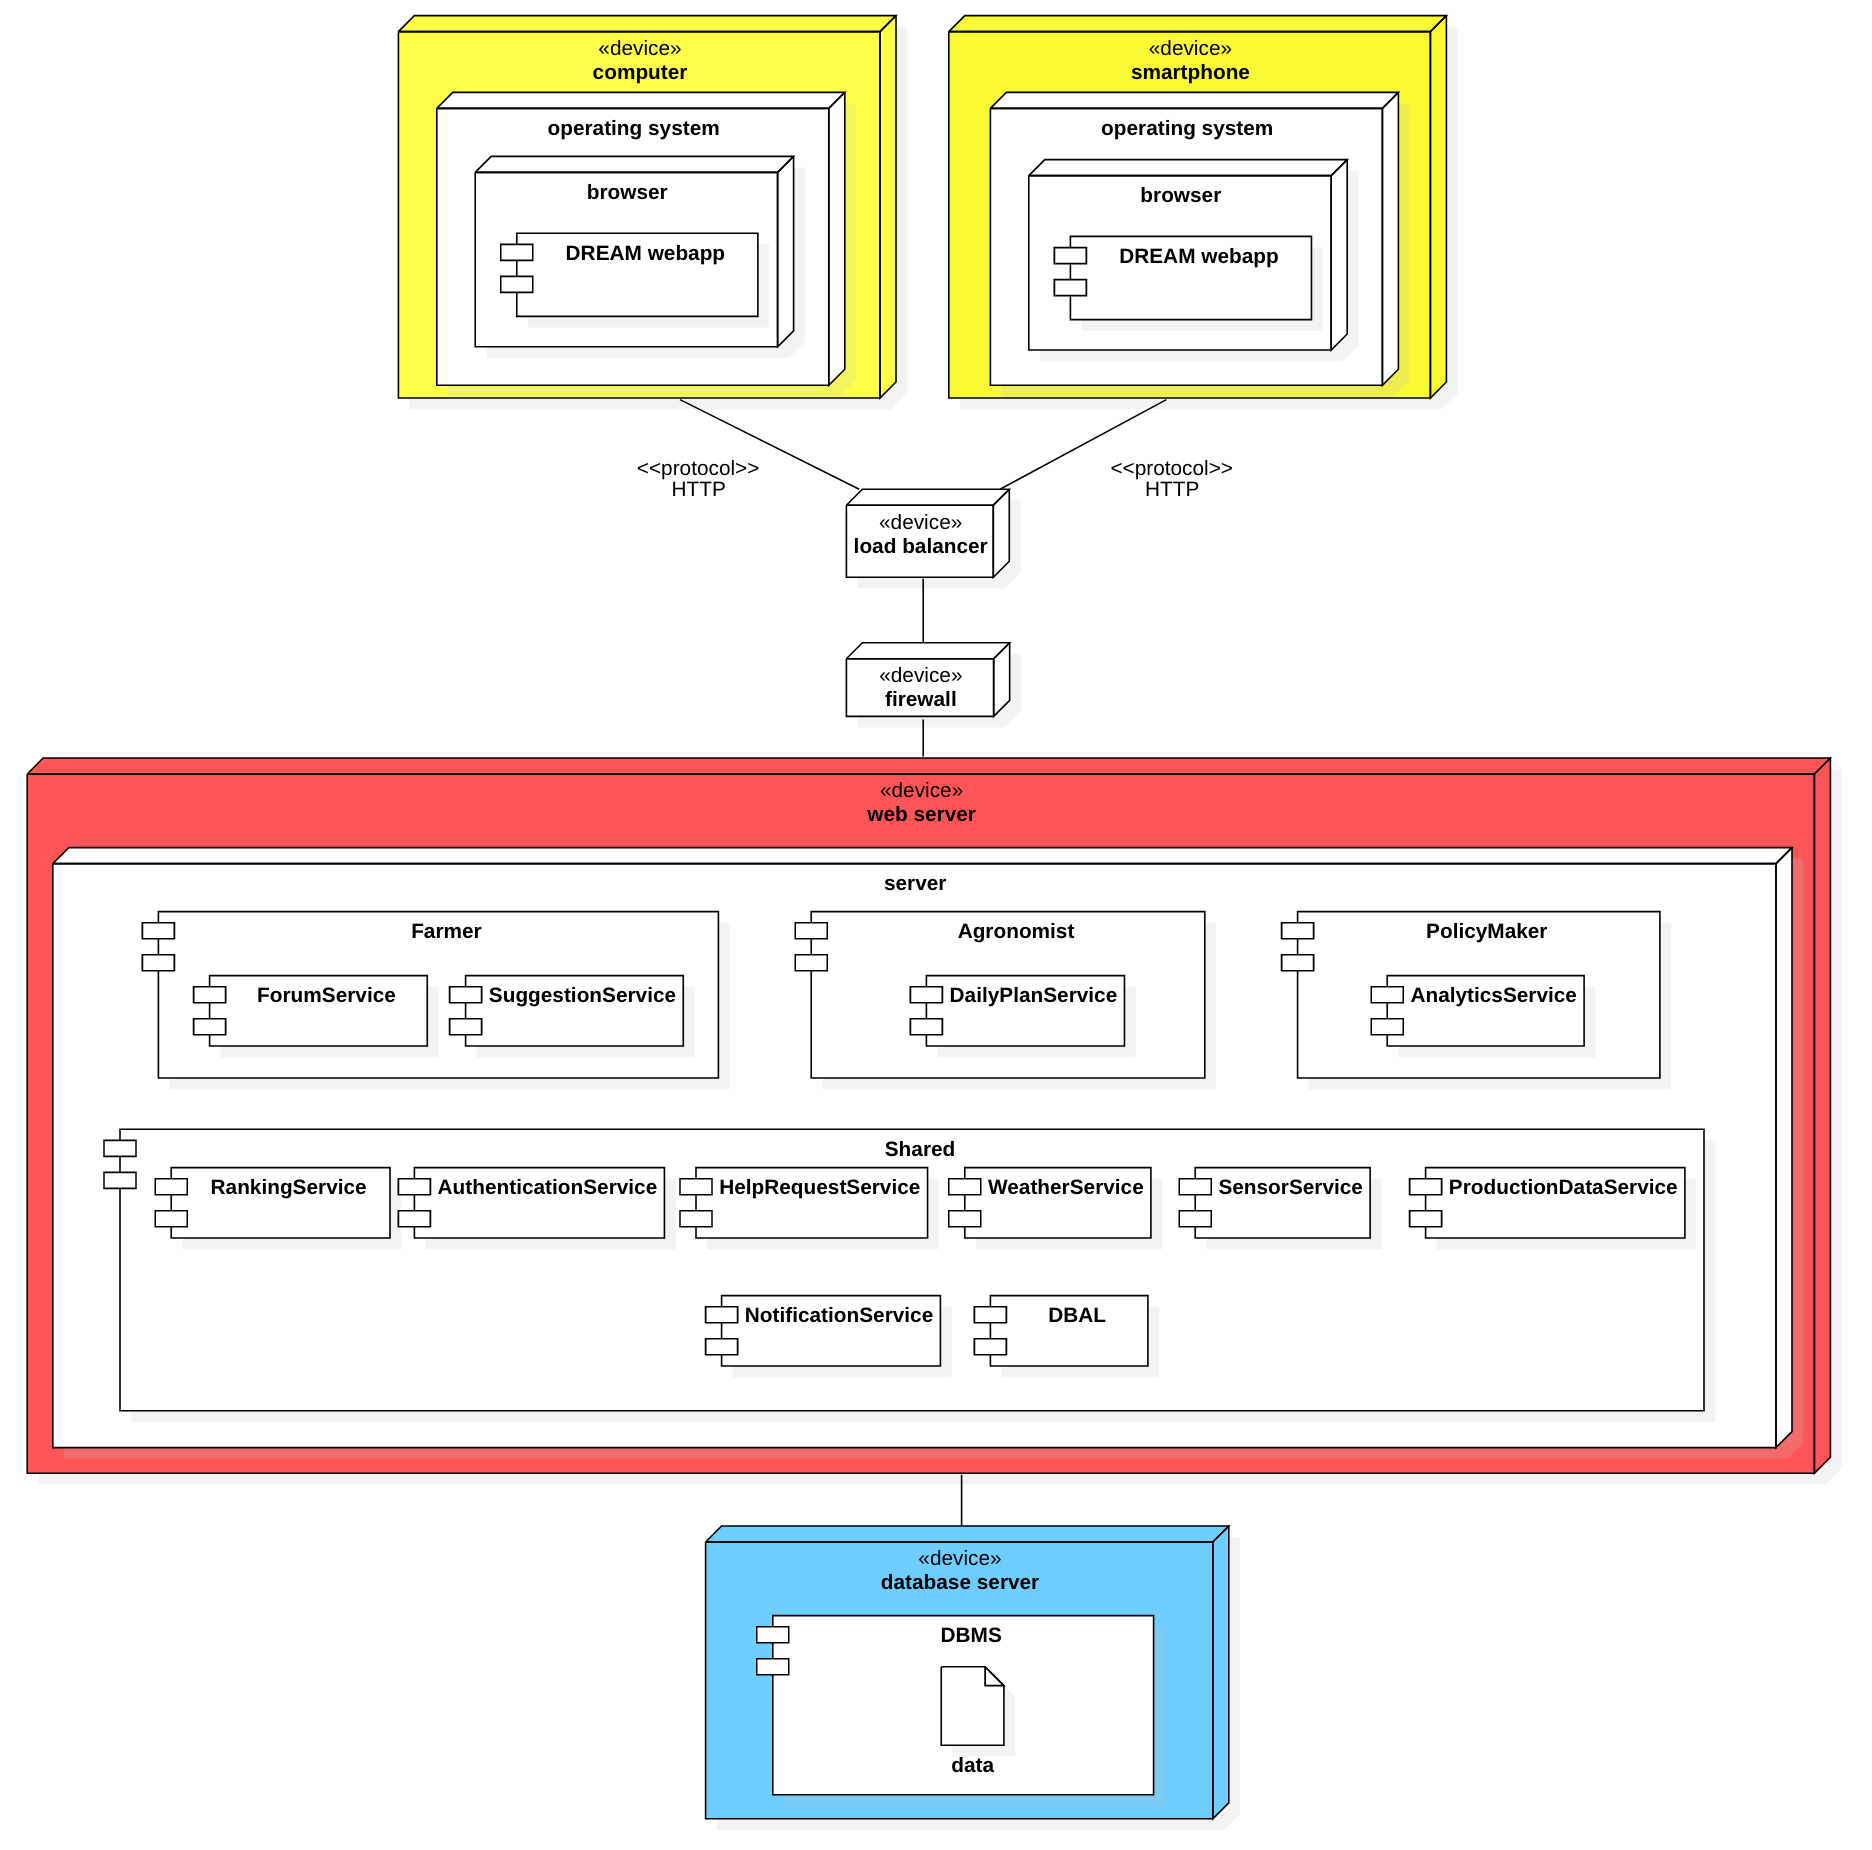
\includegraphics[trim=5cm 15cm 1cm 10cm,width=16.5cm]{diagrams/deployment_diagram.png}
\newpage
Some observations are required:
\begin{itemize}
    \item as previously specified, we opt for a 3-tiers architecture, with a web server that contains the whole business logic of the system and a database server with the data;
    \item some colours have been used for an easier visualization of the tiers;
    \item for the sake of simplicity, we have decided to represent only 2 possible clients, while the system is designed to support a much larger number;
    \item the number of web servers is more than one in order to offer faster responses and to scale better with more users;
    \item according to the amount of data to manage\footnote{see \textit{RASD - 3.3 Performance requirements} for an estimate of the storage capacity required.}, the data might be partitioned in more physical devices; for the sake of simplicity we have represented only one device since the access is hidden behind the DBAL;
    \item the architecture adopted for a scalable and secure routing of the users' requests to the servers is the FWLB (firewall load balancing), that is a \textit{deployment architecture where multiple firewall systems are placed behind Server Load Balancers}\footnote{\url{https://www.a10networks.com/blog/what-is-firewall-load-balancing-fwlb/}.}.
\end{itemize}
\subsection{Runtime view}
In this section the interactions among the components (identified at section \ref{Component view}) are shown. In order to make the presentation clearer, the UML notation of sequence diagrams is used.\\ It should be noticed that not all the use cases and scenarios identified in \textit{RASD - 3.2.3 Scenarios} and \textit{RASD - 3.2.4 Use cases} are represented here. We have decided to explicitly describe only the most relevant use cases, since in many occasions the interaction among the components is more or less the same. As a matter of fact, it often occurs that the difference lies only in the function invoked on a specific component; since all the interfaces are well-explained in the rest of this document (see section \ref{Component interfaces}), we opted to avoid this repetition.
Furthermore, the DBMS component is not represented in any sequence diagram because its interaction with the DBAL is hidden behind the software framework adopted.
\newpage
\begin{figure}[H]
   \centering
   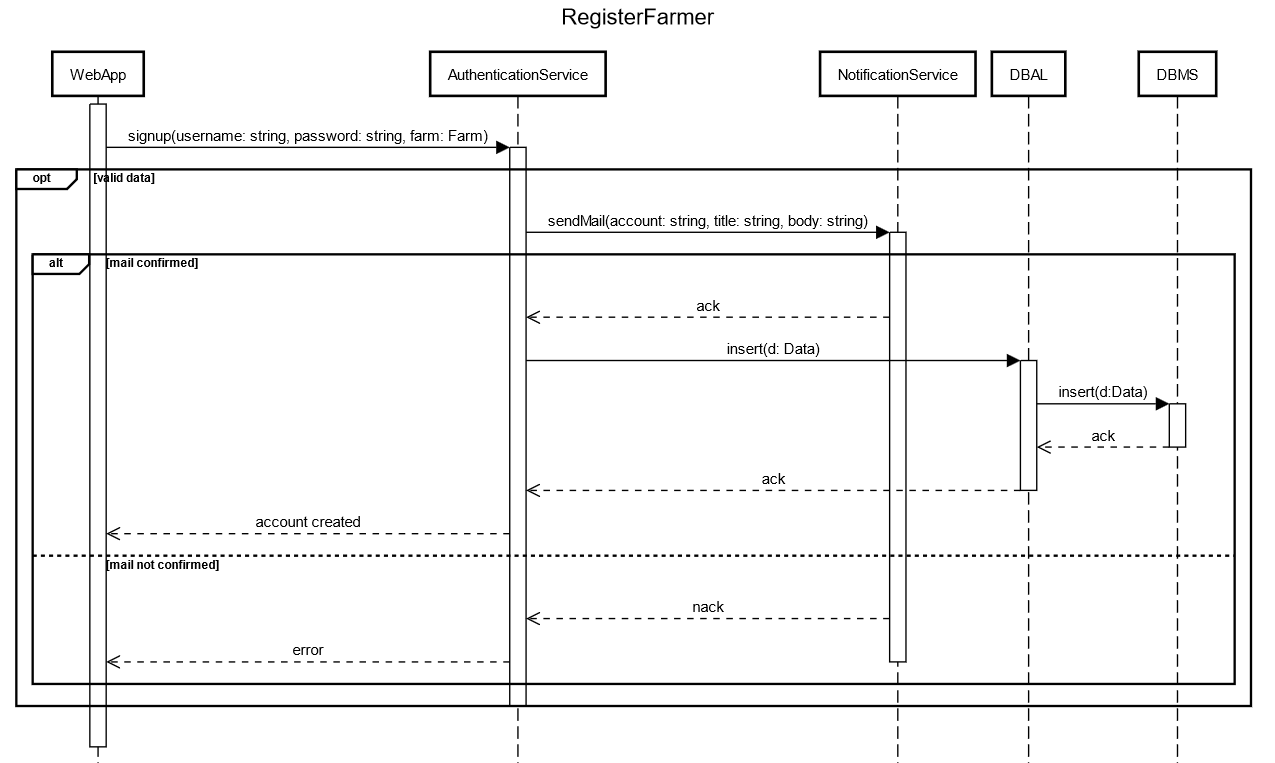
\includegraphics[scale=0.40]{diagrams/sequence diagrams/RegisterFarmer.png}
    \caption{Sequence diagram that describes the RegisterFarmer use case.}
\end{figure}
This sequence diagram describes the process of registration of a farmer in the system. The farmer invokes the signUp method on the AuthenticationService, which checks the validity of the data (length of the password, ...) and, in case data is valid, it exploits the NotificationService to send an e-mail to the farmer with a link to verify the account. In case the account is verified, the AuthenticationService stores the new account in the database and positively notifies the farmer, otherwise an error is sent.

\newpage
\begin{figure}[H]
   \centering
   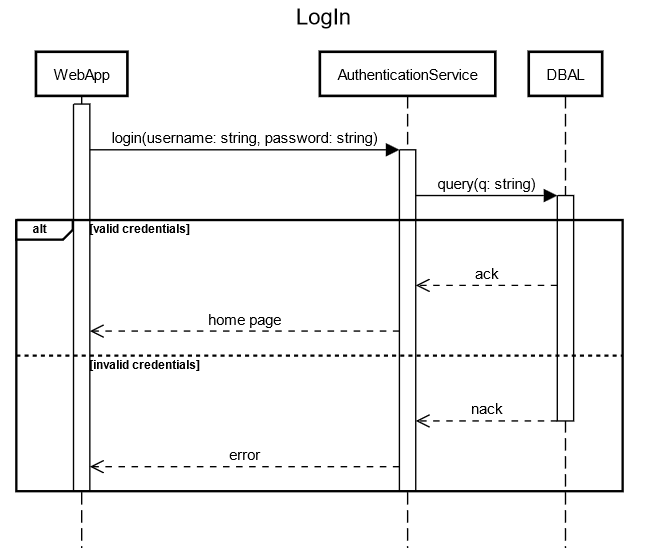
\includegraphics[scale=0.60]{diagrams/sequence diagrams/LogIn.png}
    \caption{Sequence diagram that describes the LogIn use case.}
\end{figure}

This sequence diagram describes how a user (farmer, agronomist or policy maker) can access to the system. The procedure is rather simple: the WebApp invokes the login method on the AuthenticationService which checks that the inserted credentials do not contain code for an SQL injection attack (in such a case, an error is returned to the WebApp; this branch is not represented in the diagram) and then queries the database (through the DBAL) to check whether a profile associated to the specified credentials actually exists. In such a case, the user logs in, otherwise he receives an error.\\
OBS.: from now on, checks on the data inserted by the user in order to avoid SQL injection attacks are not mentioned anymore, but they are present every time the user invokes methods of \verb|DREAM| passing arguments (since it is a functionality offered by the software framework adopted, it is not meaningful neither to represent nor to mention it every time).

\newpage
\begin{figure}[H]
   \centering
   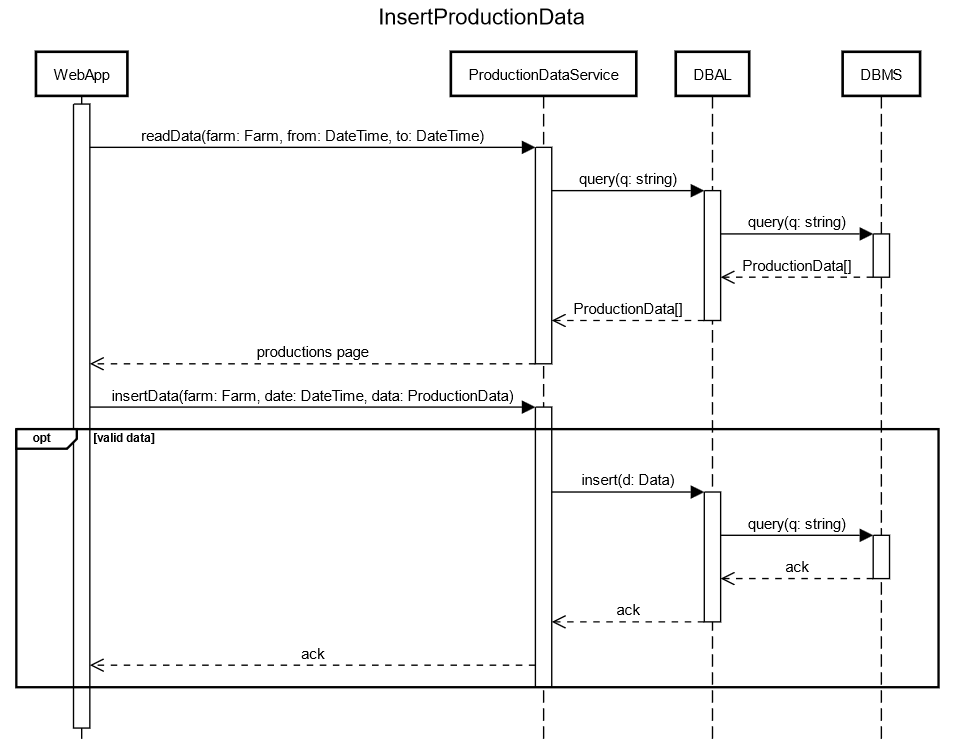
\includegraphics[scale=0.60]{diagrams/sequence diagrams/InsertProductionData.png}
    \caption{Sequence diagram that describes the InsertProductionData use case.}
\end{figure}
This sequence diagram describes the procedure through which a Farmer, starting from the home page, can insert production data in the system. According to the corresponding use case, the farmer automatically invokes the readData method when opening the "my productions" page. This call triggers an underlying retrieval of data from the database. Next, the Farmer calls insertData with all the details of the production to insert and, after a check about the validity, the data is inserted into the database and an ack is returned to the WebApp.

\newpage
\begin{figure}[H]
   \centering
   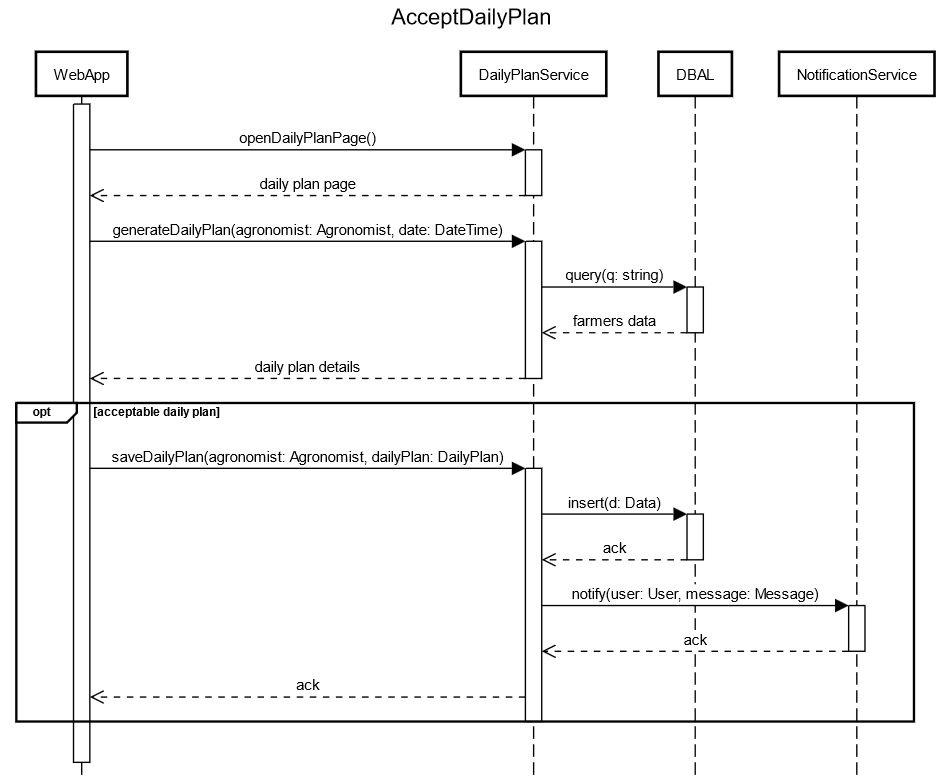
\includegraphics[scale=0.40]{diagrams/sequence diagrams/AcceptDailyPlan.png}
    \caption{Sequence diagram that describes the AcceptDailyPlan use case.}
\end{figure}
This sequence diagram describes the interactions that occur when an agronomist generates and accepts a new daily plan. First of all, the agronomist opens the daily plan page and then he selects the date of his next working day. The DailyPlanService queries the database to retrieve data about the Farmers that he needs to generate a suitable daily plan for the agronomist. In case the daily plan is acceptable to the agronomist, the WebApp invokes the saveDailyPlan method on the DailyPlanService, that stores the new daily plan in the database and then notifies the involved farmer (such interaction is not shown in the diagram).\\
OBS.: In order to modify the daily plan, specific methods are offered by the DailyPlanService. See section \ref{Component interfaces} for more details (sequence diagrams are omitted for the sake of simplicity).

\newpage
\begin{figure}[H]
   \centering
   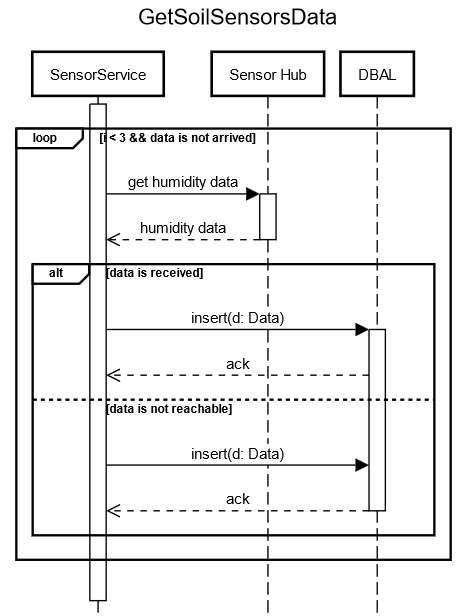
\includegraphics[scale=0.60]{diagrams/sequence diagrams/GetSoilSensorsData.png}
    \caption{Sequence diagram that describes the GetSoilSensorsData use case.}
\end{figure}
This sequence diagram describes the process with which \verb|DREAM| retrieves data from the humidity sensors (the process for the water irrigation system is analogue). Every time a timeout expires, the SensorService gets in contact with the Sensor Hub through its interface. If the data arrives, then such data is stored in the database, otherwise the SensorService stores in the database that at that specific timestamp the sensor was not reachable.

\newpage
\begin{figure}[H]
   \centering
   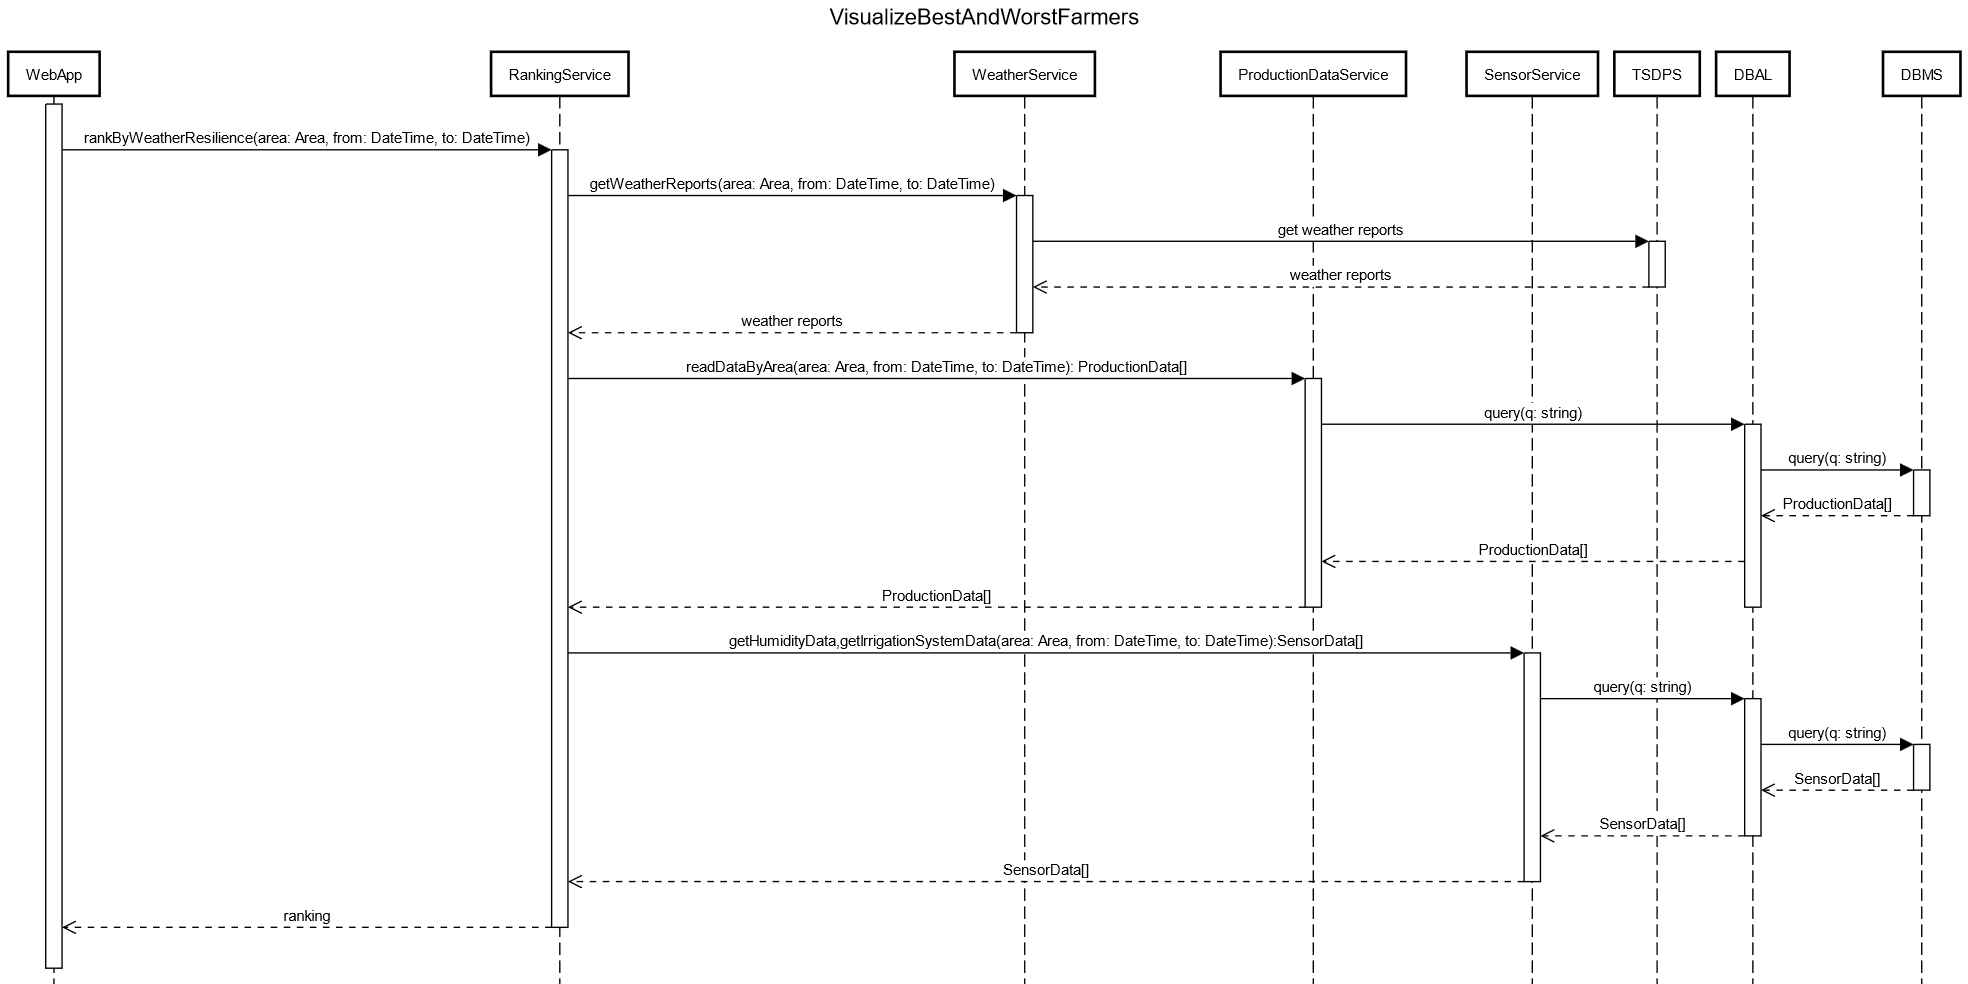
\includegraphics[scale=0.30]{diagrams/sequence diagrams/VisualizeBestAndWorstFarmers.png}
    \caption{Sequence diagram that describes the VisualizeBestAndWorstFarmers use case.}
\end{figure}
This sequence diagram describes the process that leads to the ranking of farmers. The policy maker invokes the rankByWeatherResilience method on the RankService, which exploits the WeatherService to retrieve the weather reports from the TSDPS; moreover, RankService queries the database to retrieve all the data about farmers it needs to rank them, and finally it provides the policy maker the ranking.

\newpage
\begin{figure}[H]
   \centering
   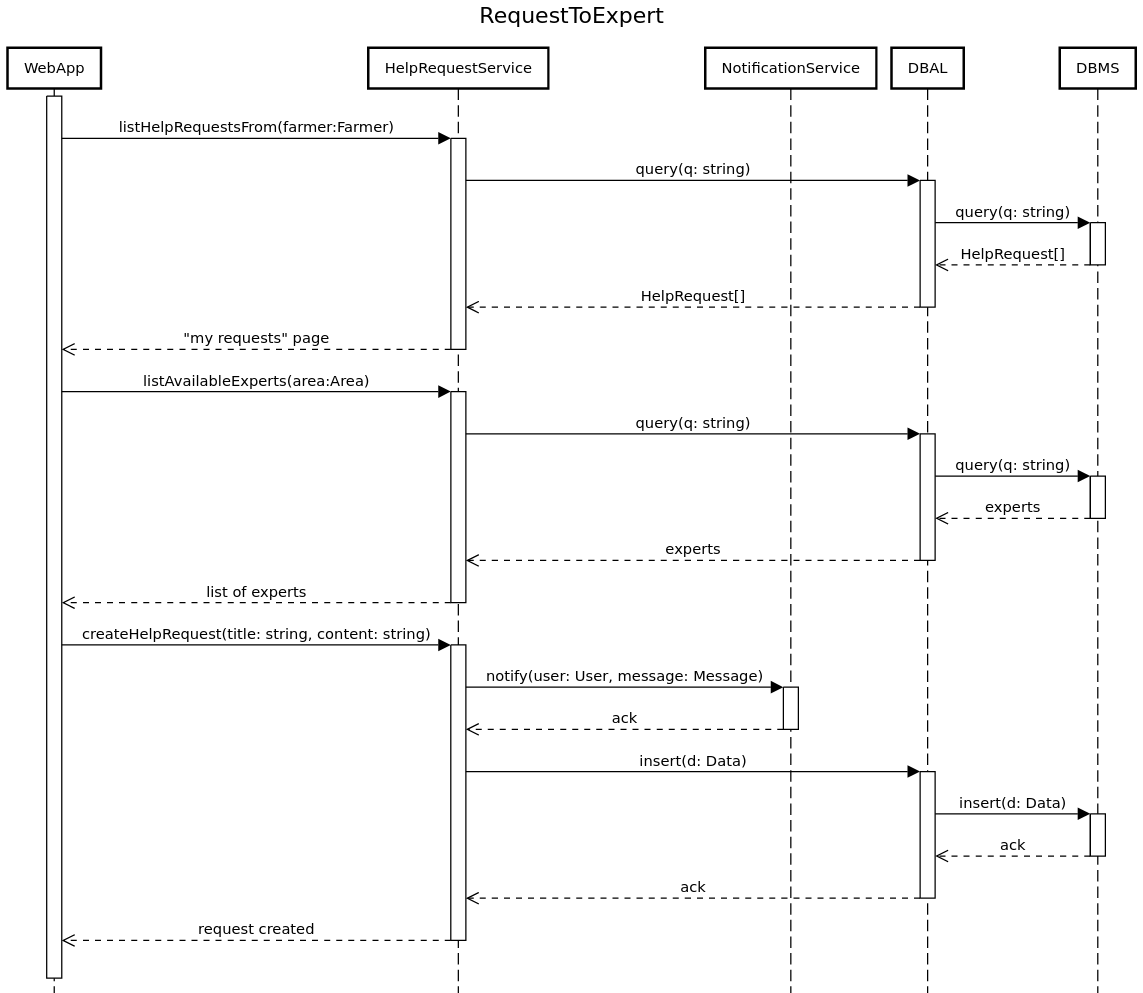
\includegraphics[scale=0.40]{diagrams/sequence diagrams/RequestToExpert.png}
    \caption{Sequence diagram that describes the RequestToExpert use case.}
\end{figure}
This sequence diagram represents the way a farmer can ask for help to an expert (agronomist or best-performing farmer). Starting from the home page, the farmer open the "my requests" page which implies a query to retrieve all the past requests of the farmer. Next, the farmer selects the expert from which he wants to receive some help and invokes the createHelpRequest method on the HelpRequestService. This service exploits the NotificationService to notify the expert, and, in case the the expert is already connected on Internet, an ack is received, the request is inserted in the database and the farmer is positively notified. It should be remarked that if the expert is not available, the system notifies the farmer that the expert will be notified as soon as he accesses \verb|DREAM| (this branch has been omitted for the sake of simplicity).

\newpage
\begin{figure}[H]
   \centering
   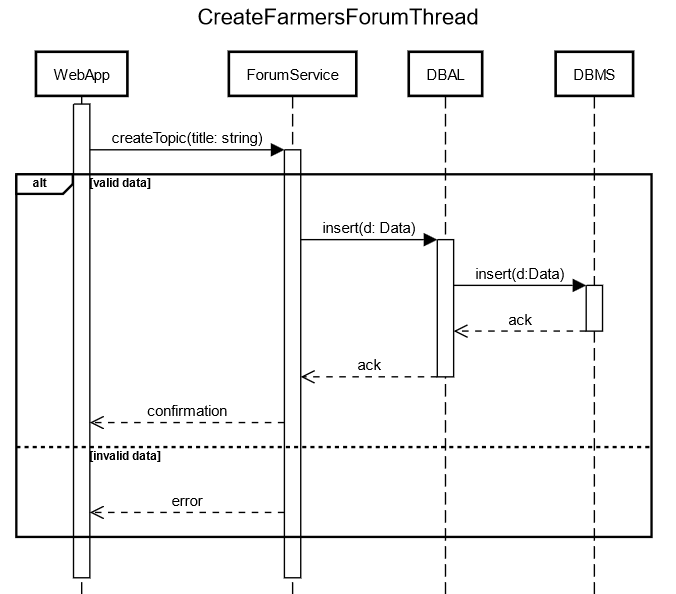
\includegraphics[scale=0.40]{diagrams/sequence diagrams/CreateFarmersForumThread.png}
    \caption{Sequence diagram that describes the CreateFarmersForumThread use case.}
\end{figure}
This diagram describes the process of creation of a new discussion thread by a farmer. It invokes the createTopic method on the HelpRequestService and, if the data inserted are valid, the service stores the information in the database and positively notifies the farmer, otherwise an error is shown.
\newpage
\subsection{Component interfaces}\label{Component interfaces}
\subsection{Selected architectural styles and patterns}
According to the definition provided by David Garlan and Mary Shaw\footnote{January 1994, CMUCS-
94-166, see "An Introduction to Software Architecture"
at \url{http://www.cs.cmu.edu/afs/cs/project/able/ftp/intro_softarch/intro_softarch.pdf}.}, \textit{an architectural style determines the vocabulary of components and connectors that can be used in instances of that style, together with a set of constraints on how they can be combined}.\\
\paragraph{Architectural style}\label{Architectural style}
Given that the tasks that \verb|DREAM| has to achieve can be perfectly reached by implementing the system as a web application, and given that the most wide-spread, standardized and successful architectural style for distributed (web) applications is the client-server one, we have decided to opt for it. As a matter of fact, every time a user (farmer, agronomist or policy maker), namely a client, has to access the system, it sends a request to \verb|DREAM|, or better, to the server of \verb|DREAM|, which processes it and answers with a response. Moreover, our choice features 3 tiers with a thin client.\\
The main advantages of this choice related to the system we have to design are:
\begin{itemize}
    \item \textbf{scalability}: the number of resources can be easily increased when needed; thanks also to the decision of adopting a 3-tiers architecture, the data is apart from the business logic, therefore the storage capacity can be increased without affecting the anything else
    \item \textbf{accessibility}: the access to the system can be done with every possible device with a browser installed and from every location as long as an Internet connection is available. Despite this characteristic might not seem as important as the others identified in the \textit{RASD}, it is relevant because it provides much flexibility to the users: given their credentials, they can access from everywhere;
    \item \textbf{security}: users can access only through their credentials; this is a method for access controls and guarantees that only authorized users are granted access.
\end{itemize}
\subsection{Other design decisions}
\paragraph{Relational database}
We have decided to opt for a relational database because they perfectly match the use case of \verb|DREAM|. As a matter of fact, according to \textit{RASD - 3.3 Performance requirements}, there is not a huge number of relations between the entities of the data, thus a graph database would be counter-productive, because of its characteristic of being schema-less; the system has not strict time requirements, therefore adopting a key-value database would be uselessly expensive; the amount of data to manage is big, but not in the order required for matching the use case of a columnar database; finally, since data has to be pre-processed by \verb|DREAM| before reaching the users (in other words we accept data exiting the database at a low level), then we avoid a document-oriented database (also because it would make us waste a lot of space).
\paragraph{Database abstraction layer}
A DBAL is useful way to abstract from the details of the specific technology adopted for the database. It allows to reduce the amount of work required for the implementation of the components to manage the data because it provides APIs that hide the technicalities of the specific database chosen.
\paragraph{Server-side framework}
For what concerns the application layer, a software framework will be used as a foundation to build upon. In addition to providing an established and streamlined development flow, the framework will provide basic interfaces to work with the HTTP protocol and handle common tasks such as webpage rendering. Additional pre-existing components will also be used to handle other generic tasks such as email sending.
\paragraph{Model view controller}
The MVC is a software design pattern that allows to design a software application using 3 different main elements:
\begin{itemize}
    \item the model, which provides all the methods to access the data of the application;
    \item the view, which allows to visualize the data in the model and deals with the interaction between the system and the user;
    \item the controller, which receives the commands of the users and carries them out by modifying the state of the other two components.
\end{itemize}
The adoption of the MVC brings many advantages during the implementation phase of \verb|DREAM|. It allows to easily organize large-size web applications, to implement graphical interfaces with less effort, to easily doing planning and maintenance and many others.
\paragraph{Multi-page application}
\verb|DREAM| will be implemented as a multi-page application; that is, every time the user changes the current page - by following a link or performing an action in the application - a request will be made to the server to provide the full content of the new page. \newline
The rationale for this choice is DREAM being an application which does not require an high degree of interactivity: a multi-page application is sufficient to satisfy all requirements while being easier to develop and maintain compared to a client-side single-page application (SPA).
\paragraph{Thin client}
For the same reasons outlined in the above paragraph, we have opted to keep most of the business logic on the server-side (thin client architecture). The server will also handle part of the presentation logic, by serving webpages that already include information relevant to the user without the need to perform further network requests, such as API calls. While this requires an higher load on the server, the use of caching techniques can keep the performance impact to a minimum without requiring extensive resources.
A minimal amount of client-side logic will be required to handle some user interface related tasks and to perform early validation on user-generated content, in order to reduce unnecessary server load.

\newpage
\section{User Interface design}
Since the front-end of the \verb|DREAM| system is a web application, the content of its user interface consists in HTML pages displayed through a browser. Some wireframes of the UI\footnote{User Interface} can be found in \textit{RASD - 3.1.1 User interface}. In this section, IFML\footnote{Interaction Flow Modeling Language, see \url{https://www.ifml.org/}} diagrams are used to show the pages composing the \verb|DREAM| website, the components contained in these pages, the events that the user can fire through his/her interaction with the UI and how these events are handled by the \verb|DREAM| system.
As explained in the previous section, the \verb|DREAM| website will be implemented as a multi-page application, which pages will be generated by server-side templating. As a consequence of this design choice, most of the UI events cause an HTTP request to the web server, which replies with an HTTP response containing the new HTML that the browser displays. As the MVC pattern is adopted - see previous section -, HTTP requests (that can be interpreted as messages produced by the UI events), are handled by the Controller components (hosted in the \verb|DREAM| server): in the following diagrams, actions of these components are displayed in grey hexagons with abstract names - these actions should be a guideline for the implementation of Controller components, but their mapping with software implementation aspects such as classes or methods is not discussed here.
The following diagrams are referred to the PC version of the website; adjustments for the mobile version of the website - due to visualization issues - are specified in the textual descriptions of the diagrams.

\subsection {General Overview}
\begin{figure}[H]
   \centering
   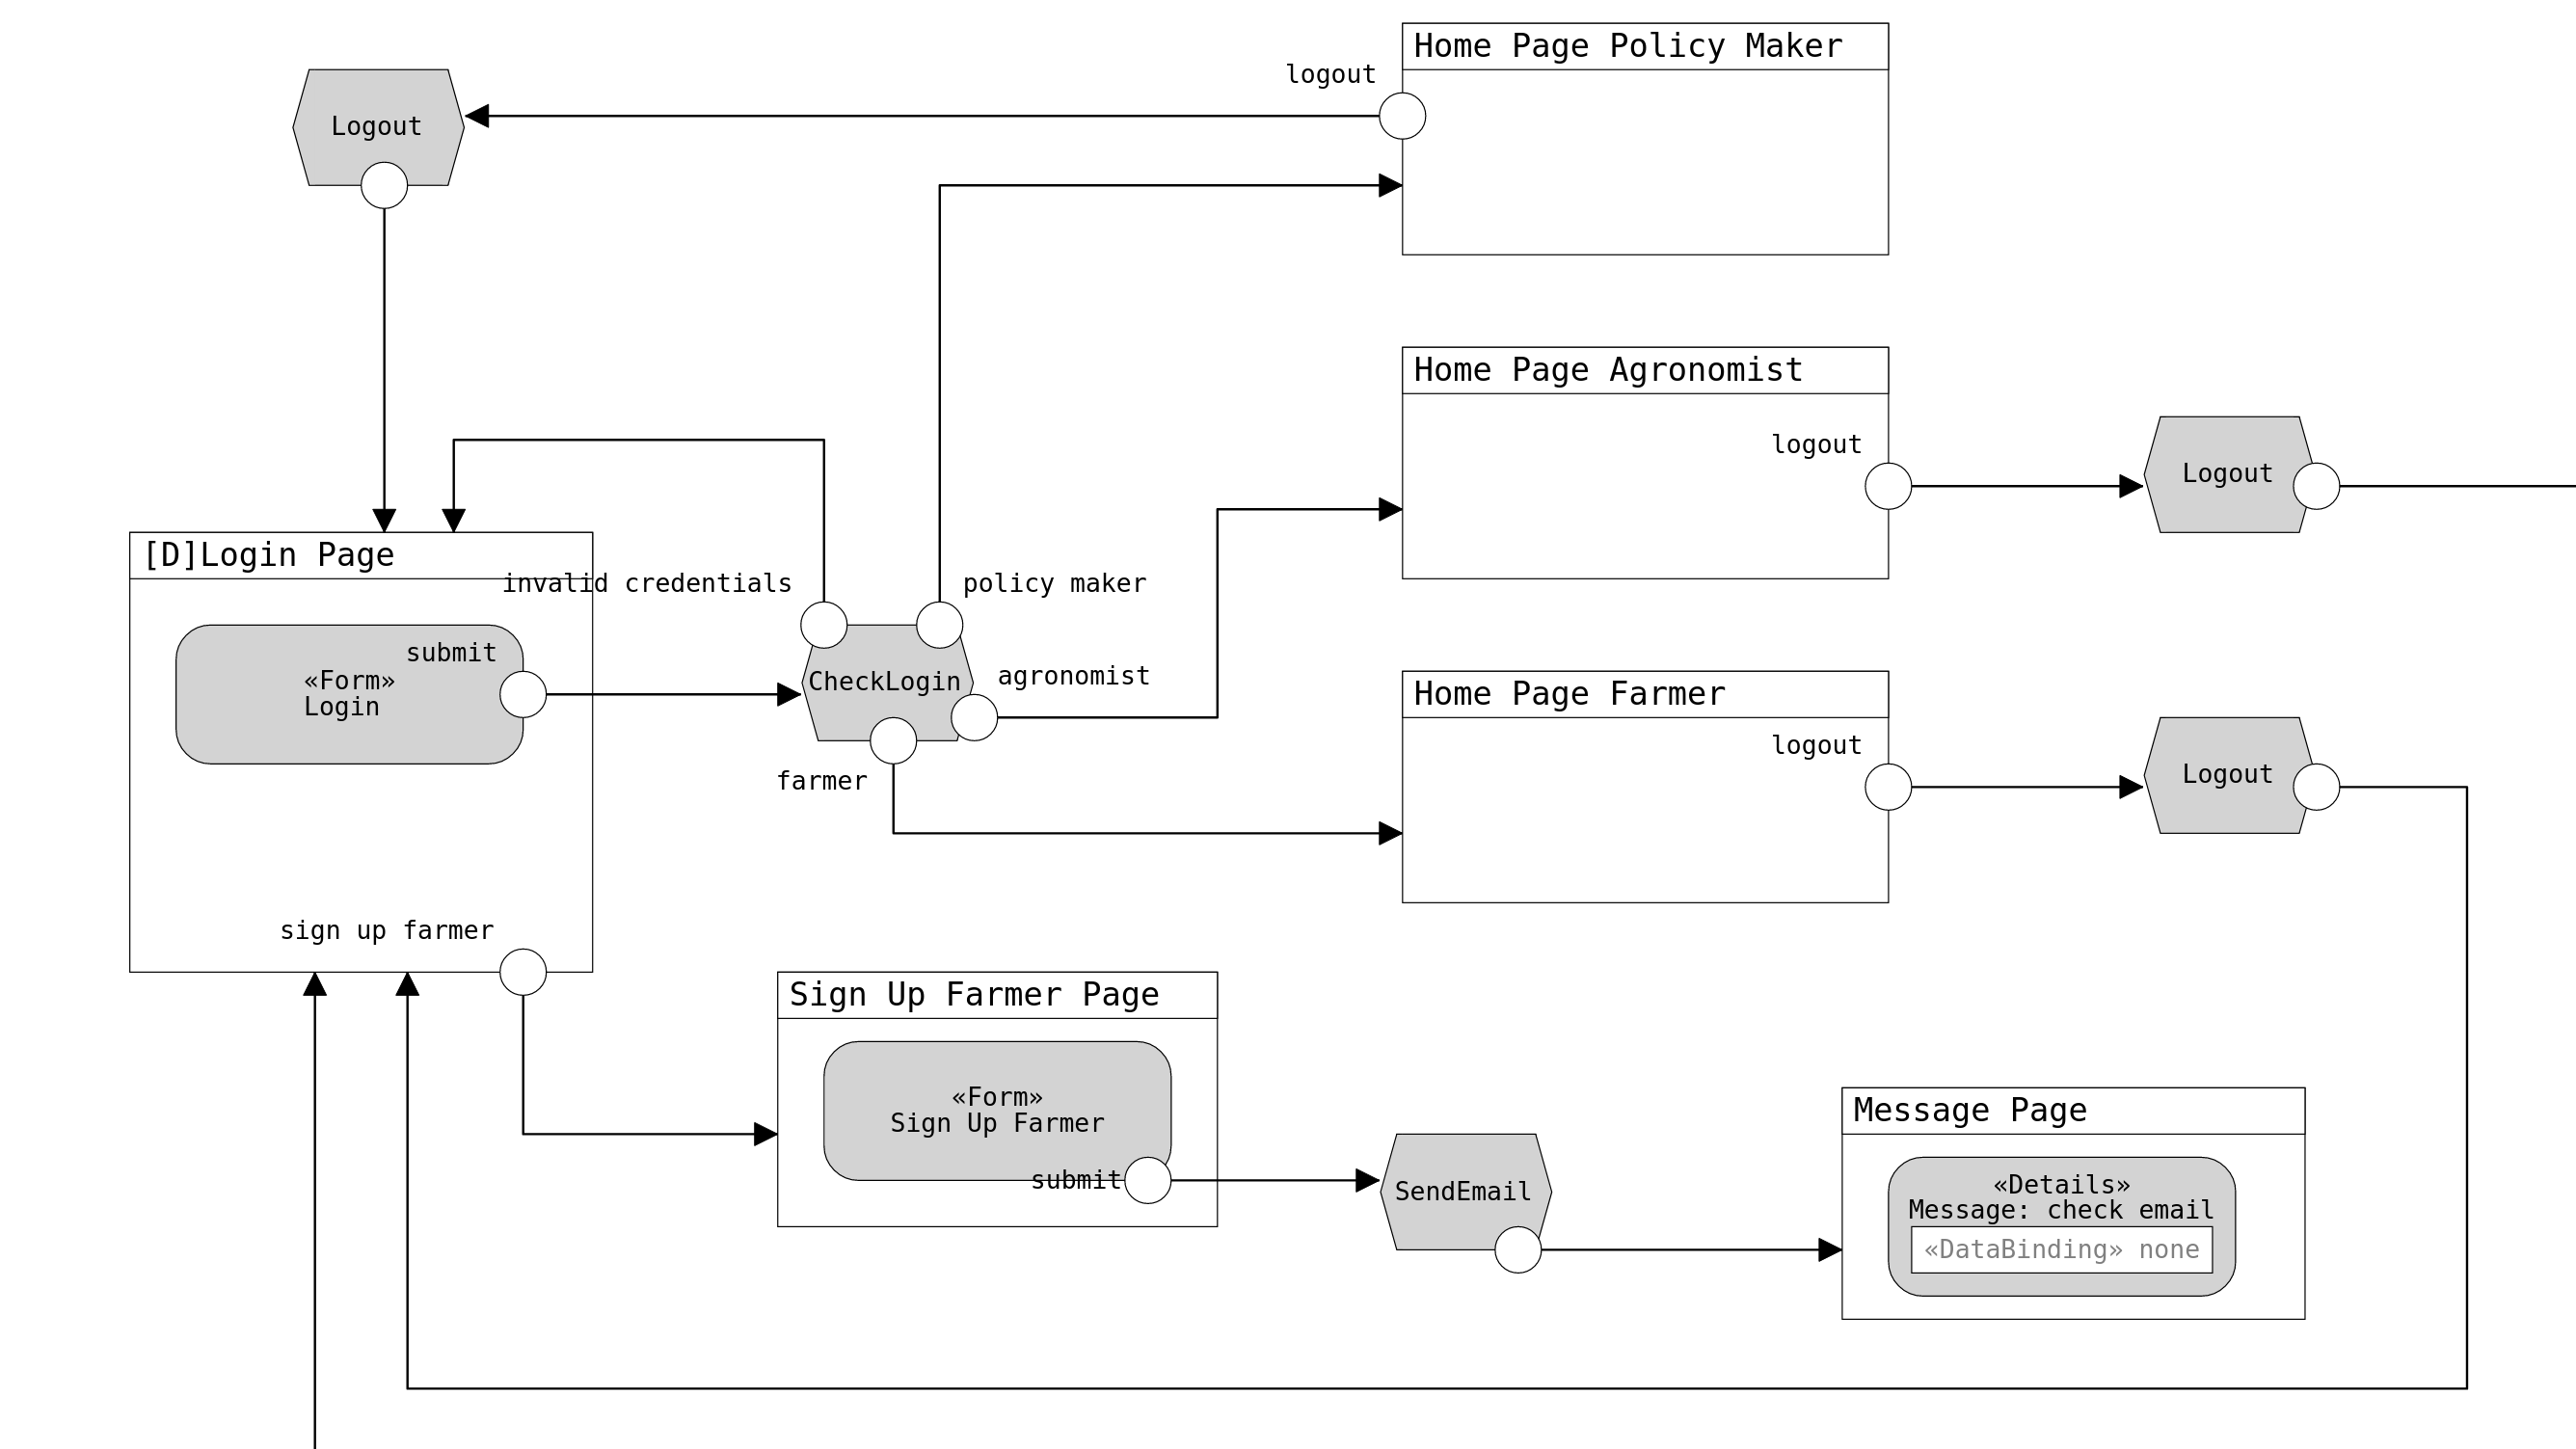
\includegraphics[scale=0.15]{diagrams/ui diagrams/login.png}
    \caption{IFML diagram with login and home pages.}
\end{figure}
The \verb|DREAM| website has a public landing page - Login page - which contains a form for logging in the system and a button for accessing a registration page for farmers accessing the system for the first time.
By submitting the form for logging in, if the credentials inserted are correct - CheckLogin action -, the user is shown the home page corresponding to his role - either farmer, agronomist or policy maker.\footnote{See \textit{RASD - 3.2.4 Use cases}, Use Case 3.}
If the user clicks on the button for signing up as a farmer, he/she is shown a new page containing a form for inserting his/her personal and working data and the credentials he/she wants to use to access the \verb|DREAM| system. By submitting this form, the user is sent an email containing a link for confirming the email address inserted and is shown a new page with a message asking him/her to check the email.\footnote{See \textit{RASD - 3.2.4 Use cases}, Use Case 1.}
Each page of the website, except for Login Page, Sign Up Farmer Page and Message Page, contains a button for logging out, that, if selected, brings to the Login Page.
\newpage
\subsection{Farmer Interface}
The Home Page for farmers contains a menu, from which the user can access the five sections of the interface: "My Production", "Weather Forecasts", "Suggestions", "My Requests", "Forum".
If the farmer is marked as best-performing, the menu shows also the menu entry for a sixth section, "My Replies", as best-performing farmers can be asked questions by other farmers, as agronomists do.\newline
If there are any notifications for the farmer - e.g., a request he/she made has been answered and he/she has not read the answer yet -, they are displayed in the Home Page.\newline
All pages represented in the diagram contain the main menu (not displayed in the diagram for the sake of simplicity), so that the user can freely navigate from one section to another without passing through the Home Page. 

\begin{sidewaysfigure}
    \centering
     \includegraphics[scale=0.07]{diagrams/ui diagrams/farmer/farmer.png}
    \caption{IFML diagram for the farmer portion of the interface.}
\end{sidewaysfigure}
\newpage
\subsubsection{"My Production" section}
\begin{figure}[H]
    \centering
     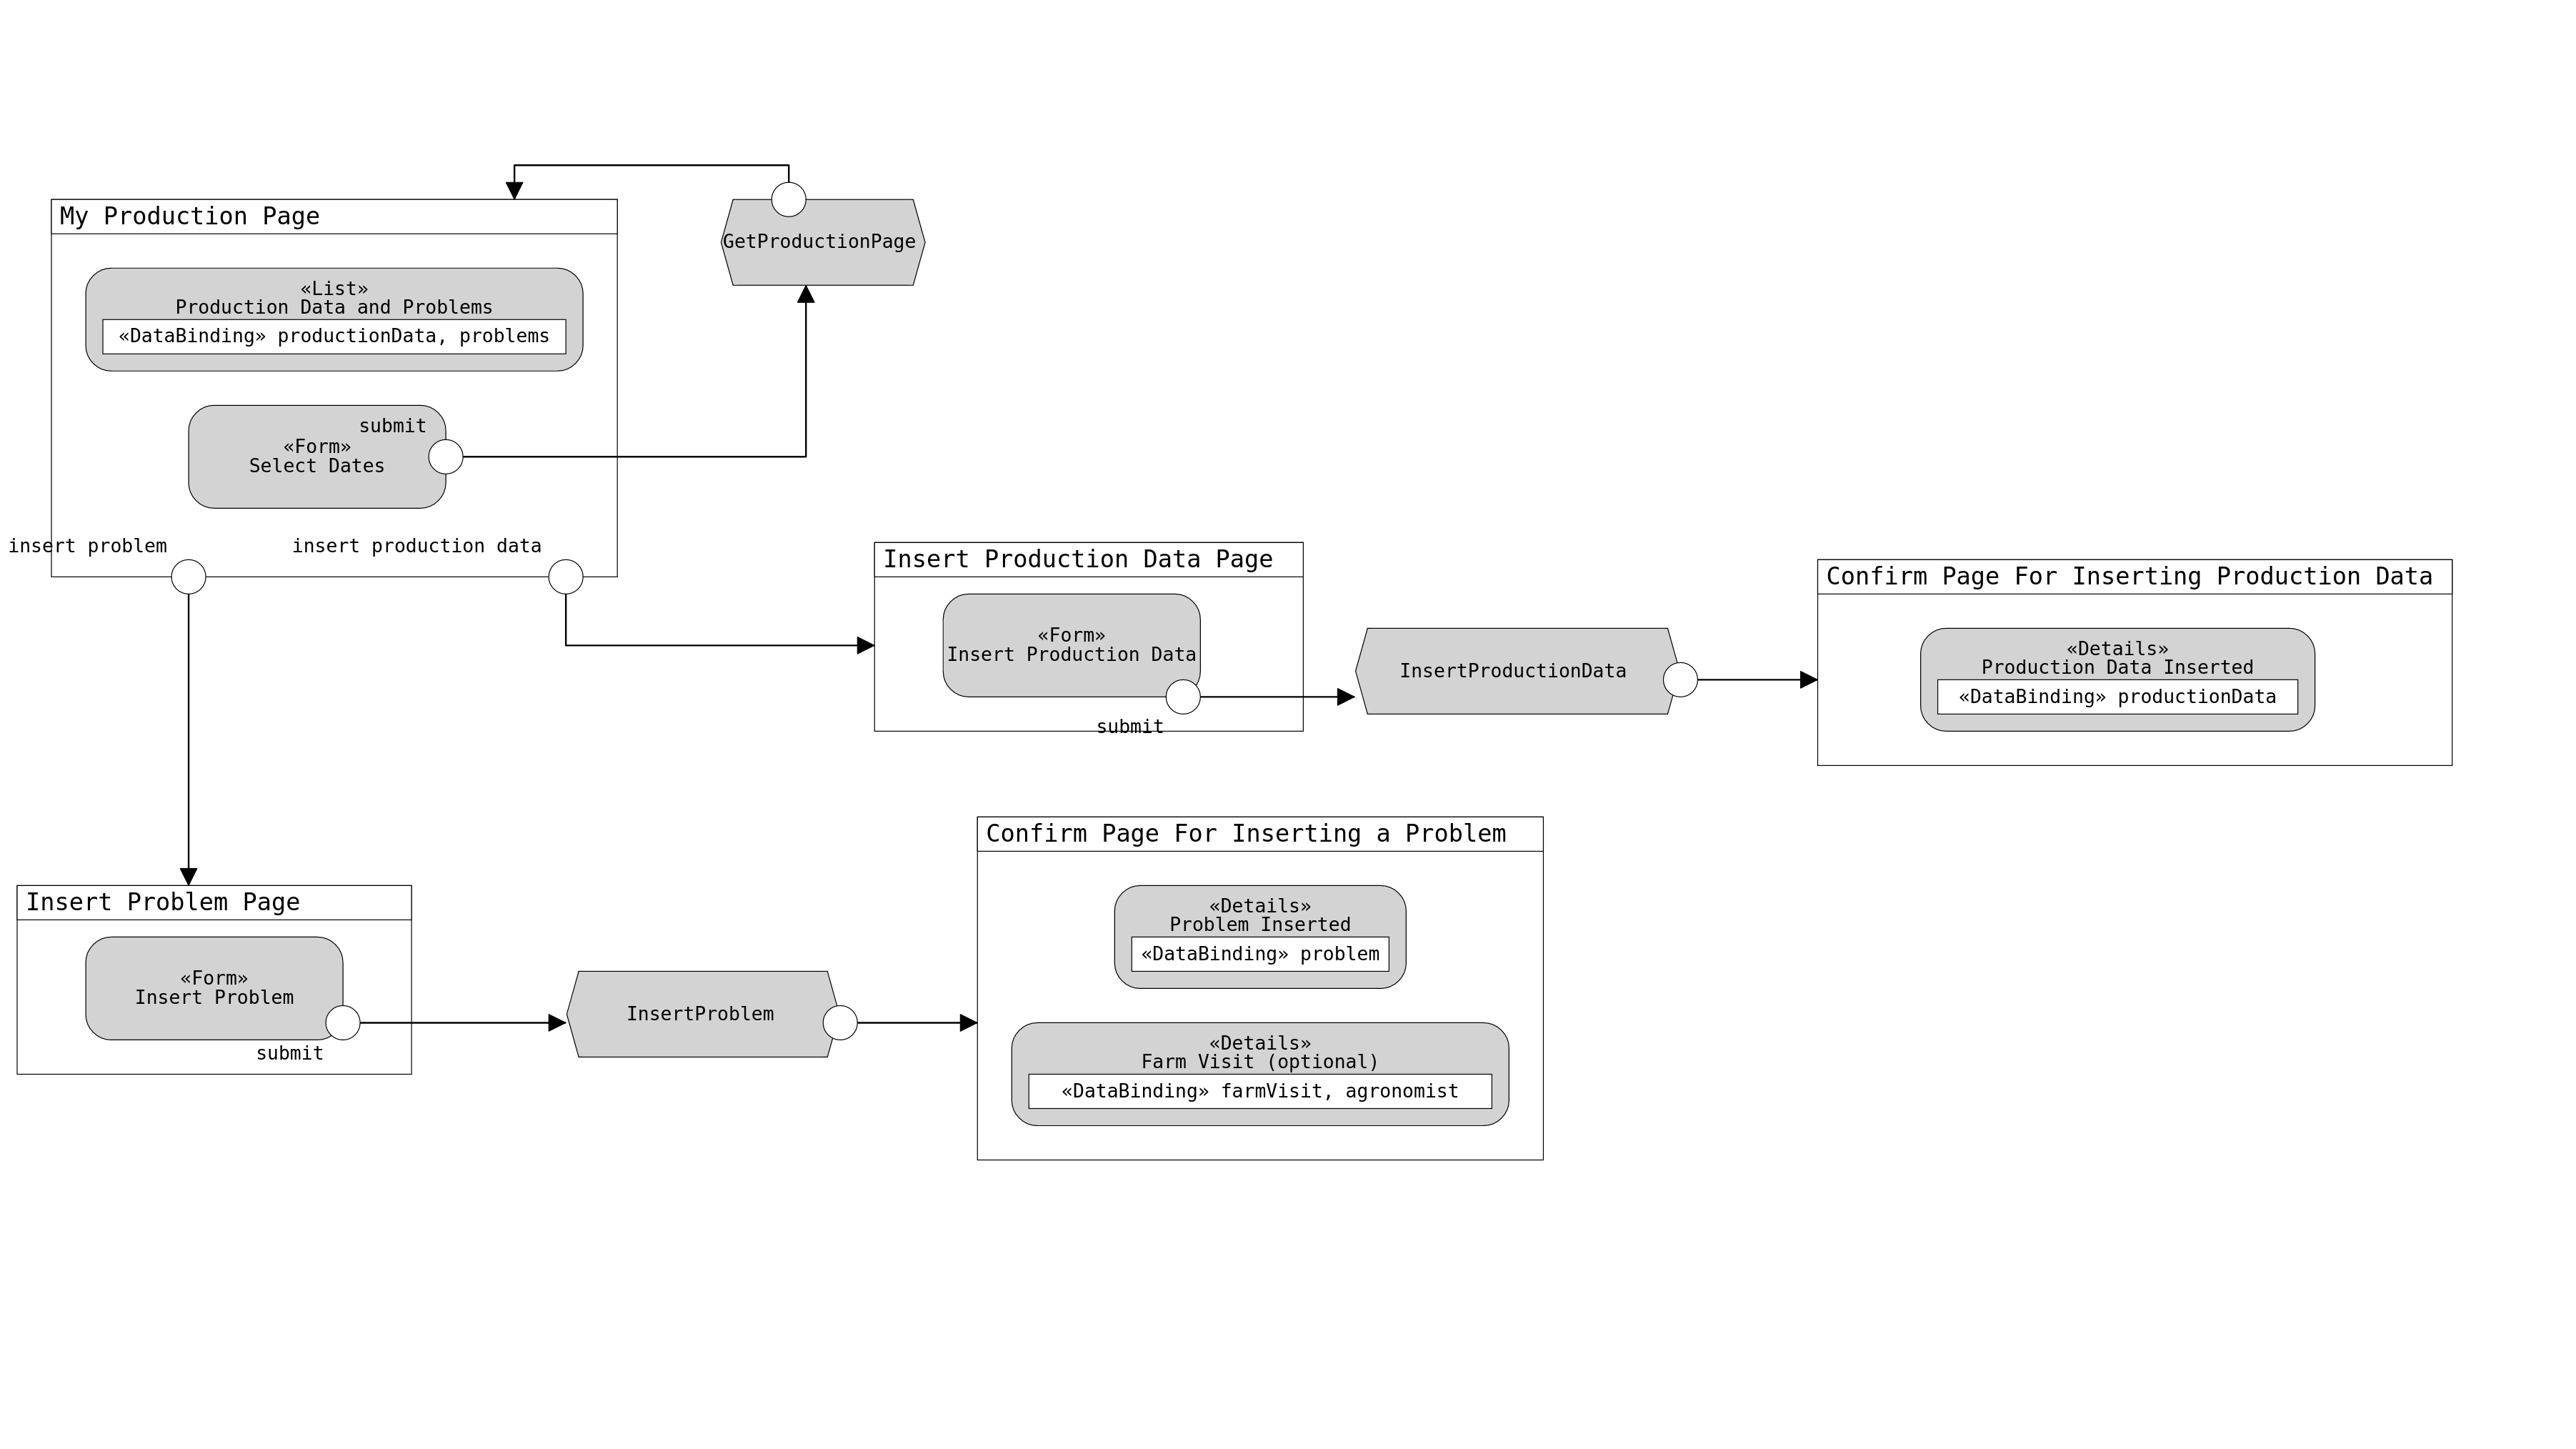
\includegraphics[scale=0.1]{diagrams/ui diagrams/farmer/my production.png}
    \caption{IFML diagram for the "My Production" section of the farmer interface.}
\end{figure}
By selecting the "My Production" entry of the main menu, the user is displayed the My Production Page, which contains a list of the production data and problems inserted by the user in descending temporal order. In the PC version of the website, only the last 20 production data and/or problems inserted are displayed, while in the mobile version of the website only the last 10 are displayed. The page also displays a "Previous" and a "Next" buttons, that allow the user to change the set of the 20 items displayed by going back or forward in time, and a form for selecting the starting and ending dates of the items to visualize (always considering the limit of 20 or 10 items that can be visualized at the same time).\footnote{See \textit{RASD - 3.2.4 Use cases}, Use Case 4.} The My Production page also contains a button "Insert Production Data", a button "Insert Problem" and a button "Back" that takes to the Home Page - back buttons are not displayed in the diagrams for the sake of simplicity-.\newline
By selecting the "Insert Production Data" button in the My Production Page, the user is displayed the Insert Production Data page, which contains a form for inserting the production data for a work day. By submitting this form, the user is displayed a confirmation page, that shows the data inserted together with a confirmation message.\footnote{See \textit{RASD - 3.2.4 Use cases}, Use Case 5.}\newline
By selecting the "Insert Problem" button in the My Production Page, the user is displayed the Insert Problem Page, which contains a form for inserting a description of a problem the user is facing and for optionally requesting the visit of an agronomist as soon as possible. By submitting this form, the user is displayed a confirmation page, that shows the problem inserted, a confirmation message, and, if he/she requested the agronomist's visit, the scheduled date of the visit and the agronomist who will perform the visit.\footnote{See \textit{RASD - 3.2.4 Use cases}, Use Case 6.}\newline
All the pages Insert Production Data, Insert Problem, Confirm Page For Inserting Production Data, Confirm Page for Inserting a Problem contain a "Back" button that takes to the My Production Page.

\subsubsection{"Weather Forecasts" section}
\begin{figure}[H]
    \centering
     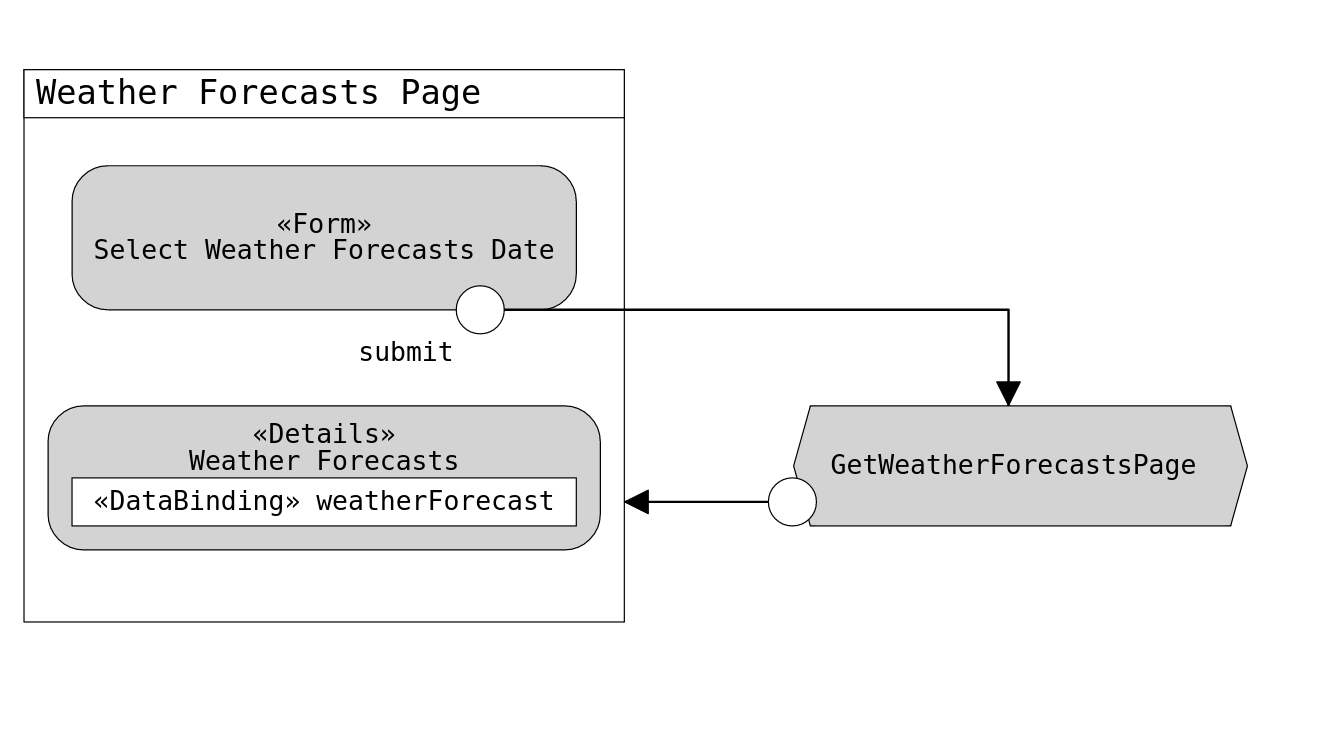
\includegraphics[scale=0.15]{diagrams/ui diagrams/farmer/weather forecasts.png}
    \caption{IFML diagram for the "Weather Forecasts" section of the farmer interface.}
\end{figure}
By selecting the "Weather Forecasts" entry of the main menu, the user is displayed the Weather Forecasts Page, which contains an input field for selecting the date of the forecasts to visualize. When the user chooses the date, the weather forecasts are shown in the same page if the website is visualized from a PC, while they are shown in a different page if the website is visualized from a mobile device.\footnote{See \textit{RASD - 3.2.4 Use cases}, Use Case 19.}\newline
A "Back" button in the Weather Forecasts Page brings to the Farmer Home Page.

\subsubsection{"Suggestions" section}
\begin{figure}[H]
    \centering
     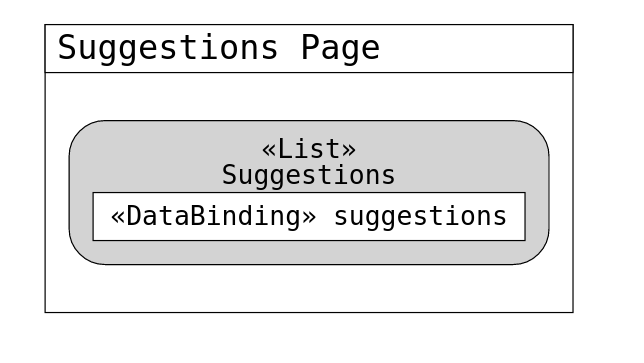
\includegraphics[scale=0.2]{diagrams/ui diagrams/farmer/suggestions.png}
    \caption{IFML diagram for the "Suggestions" section of the farmer interface.}
\end{figure}
By selecting the "Suggestions" entry of the main menu, the user is displayed the Suggestions Page, where some suggestions tailored for him/her are displayed.\footnote{See \textit{RASD - 3.2.4 Use cases}, Use Case 20.}
A "Back" button in this page brings to the Farmer Home Page.

\subsubsection{"My Requests" section}
\begin{figure}[H]
    \centering
     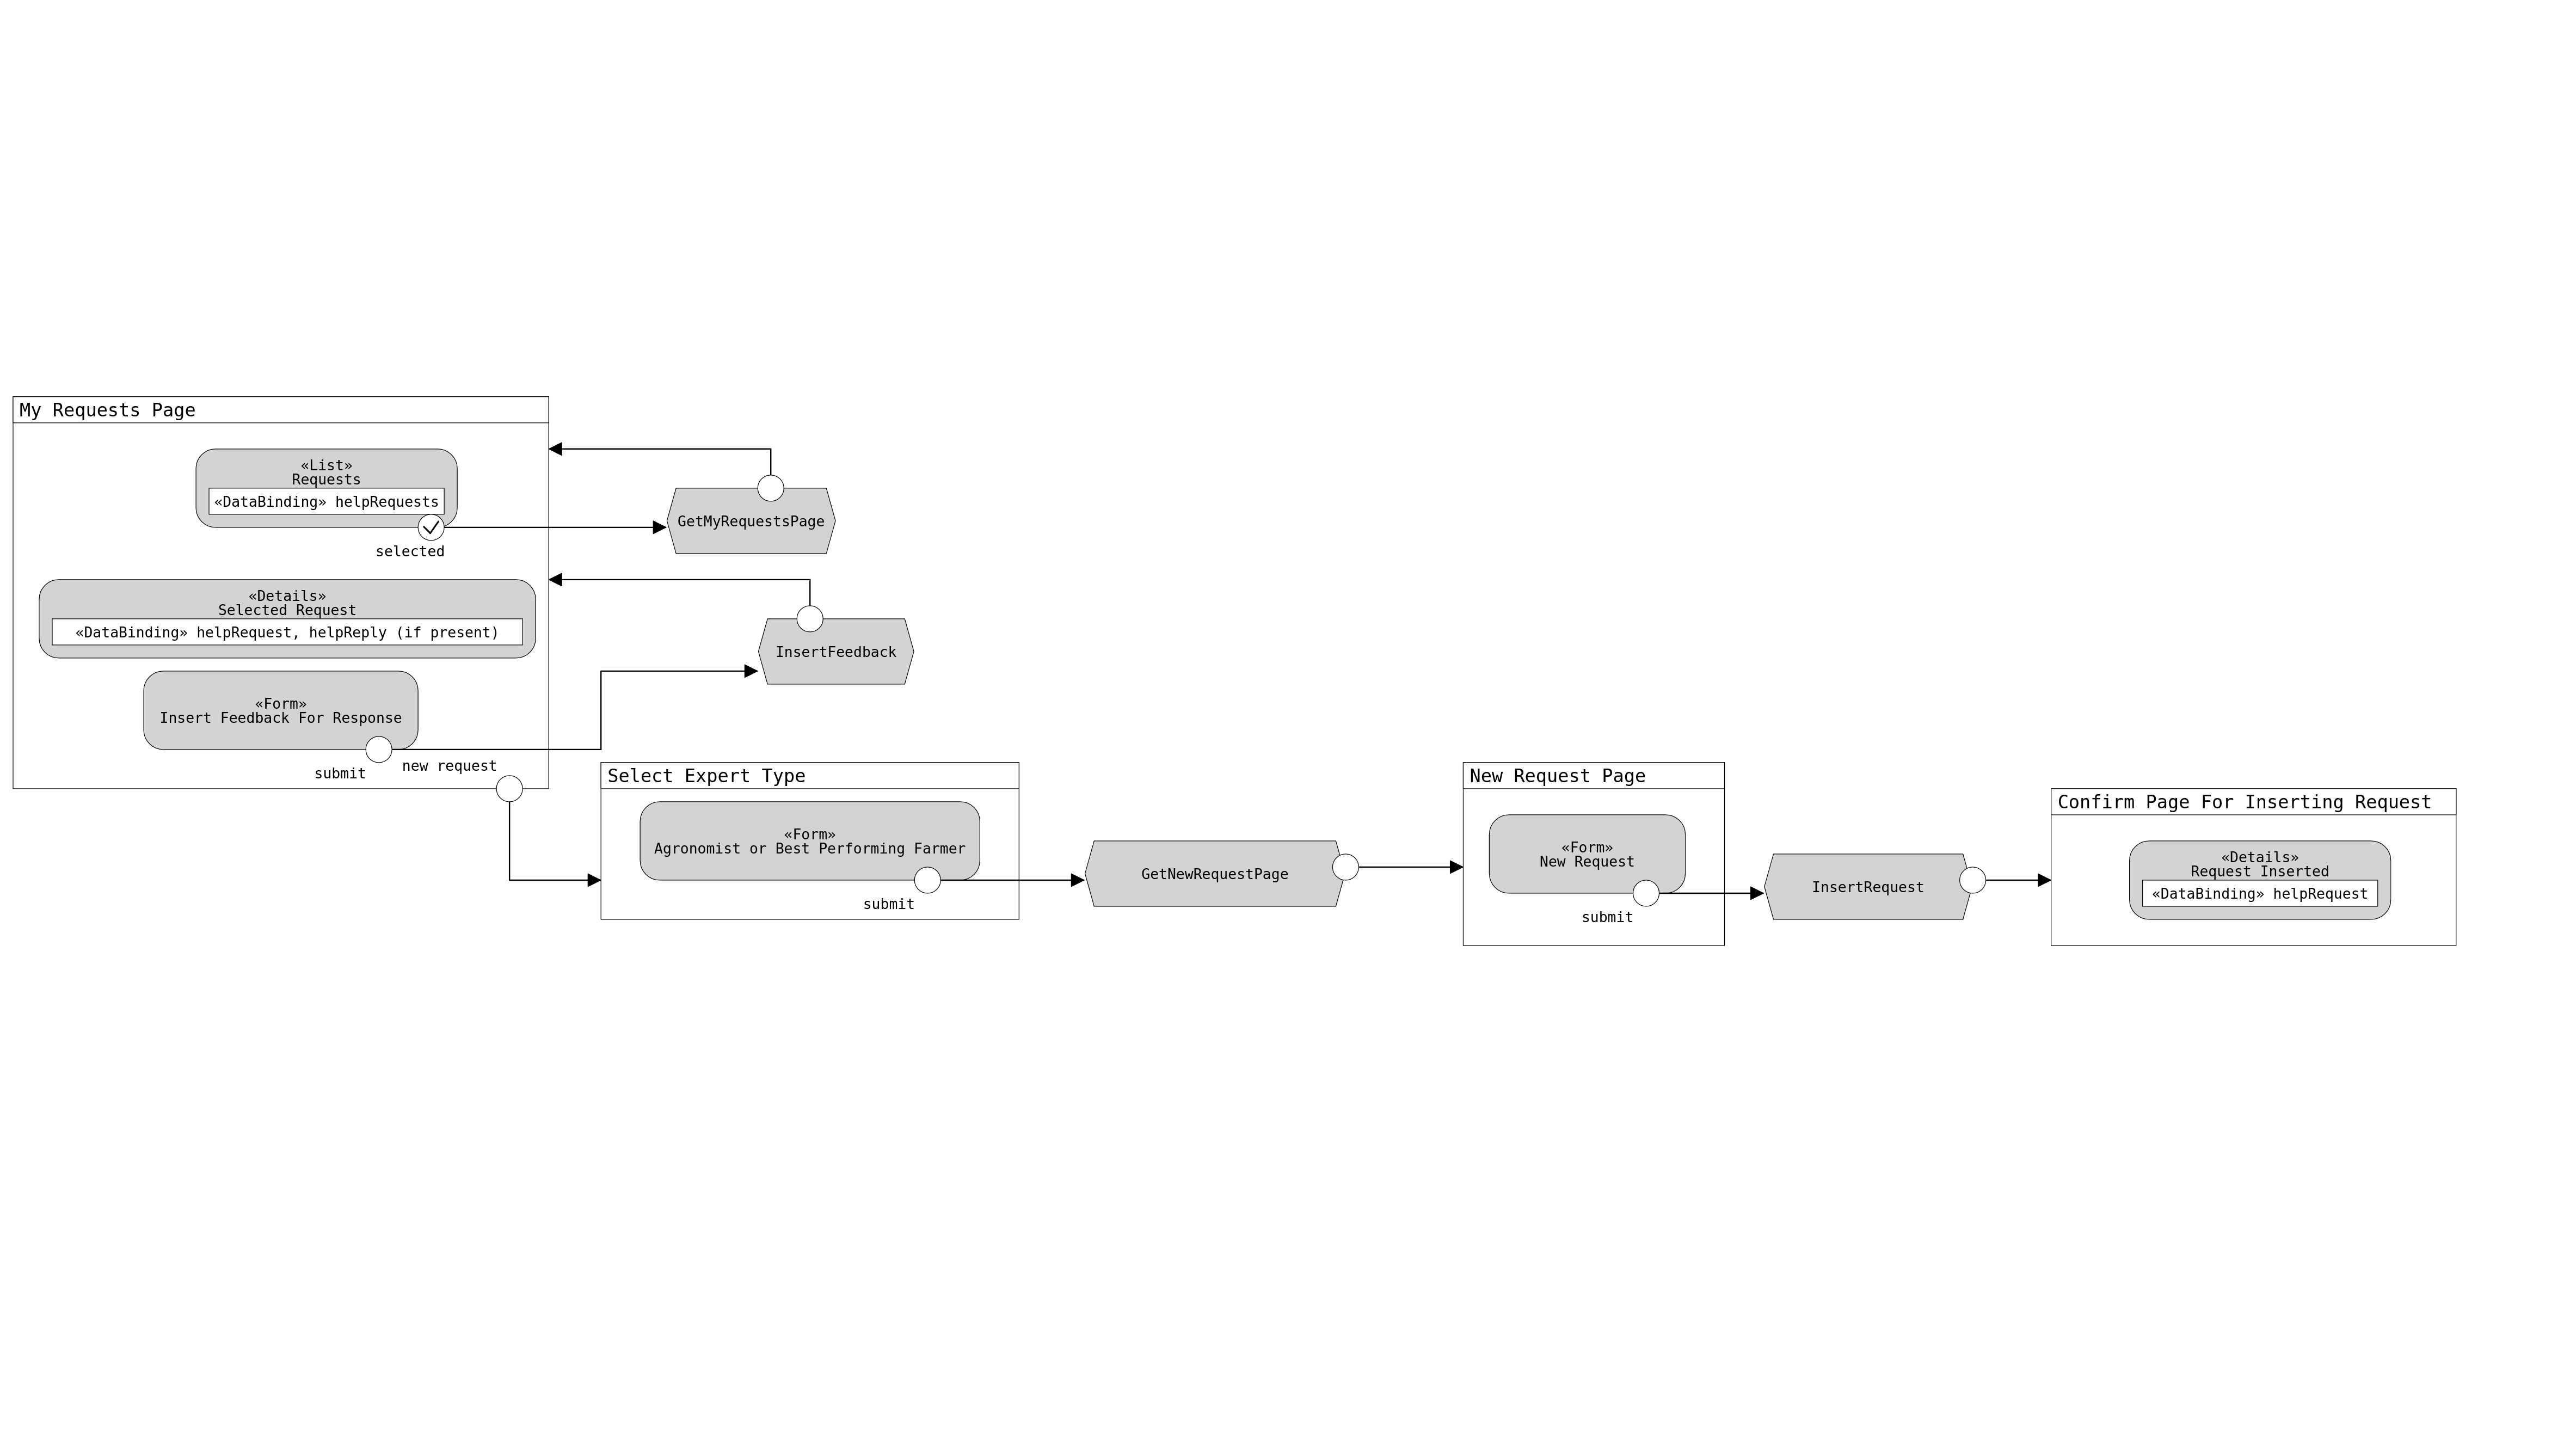
\includegraphics[scale=0.1]{diagrams/ui diagrams/farmer/my requests.png} 
    \caption{IFML diagram for the "My Requests" section of the farmer interface.}
\end{figure}
By selecting the "My Requests" entry of the main menu, the user is displayed the My Requests Page, which contains a list of the requests issued by him/her, ordered in descending temporal order. For each request, the title, the date and the receiver of the request are shown. As for the production data items and problems in the My Production Page, only the last 20 requests are shown in the PC version of the website, while only the last 10 ones are displayed in the mobile version of the website, and a "Previous" and "Next" button are present to visualize other requests. Requests which have been already replied are marked to distinguish them from unanswered ones, and requests which corresponding reply has not been read yet by the farmer are highlighted. \newline
By selecting a request in the list, the farmer is shown in the My Requests Page also the text of the request, and if the request have been replied also the text of the response. If the farmer has already inserted a feedback for the response, it is shown, otherwise an input field for inserting such feedback is shown.\footnote{See \textit{RASD - 3.2.4 Use cases}, Use Case 24.} If the website is visited from a mobile device, the details about the request and the response are visualized in a different page from the My Production Page. \newline
In the My Production Page, a "New Request" button is present, and if the user selects it, he/she is shown a page for choosing whether to submit the request to an agronomist or to a best-performing farmer. After this choice, the user is displayed a New Request Page, containing a form for creating a new request. After submitting this form, the user is displayed a confirmation page, that shows the details of the request inserted together with a confirmation message.\footnote{See \textit{RASD - 3.2.4 Use cases}, Use Case 22.}
\newline
In the My Requests page there is a "Back" button that brings to the Farmer Home Page; in the New Request Page and in the Confirm Page For Inserting Request there is a "Back" button that brings to the My Requests Page.

\subsubsection{"My Replies" section}
\begin{figure}[H]
    \centering
     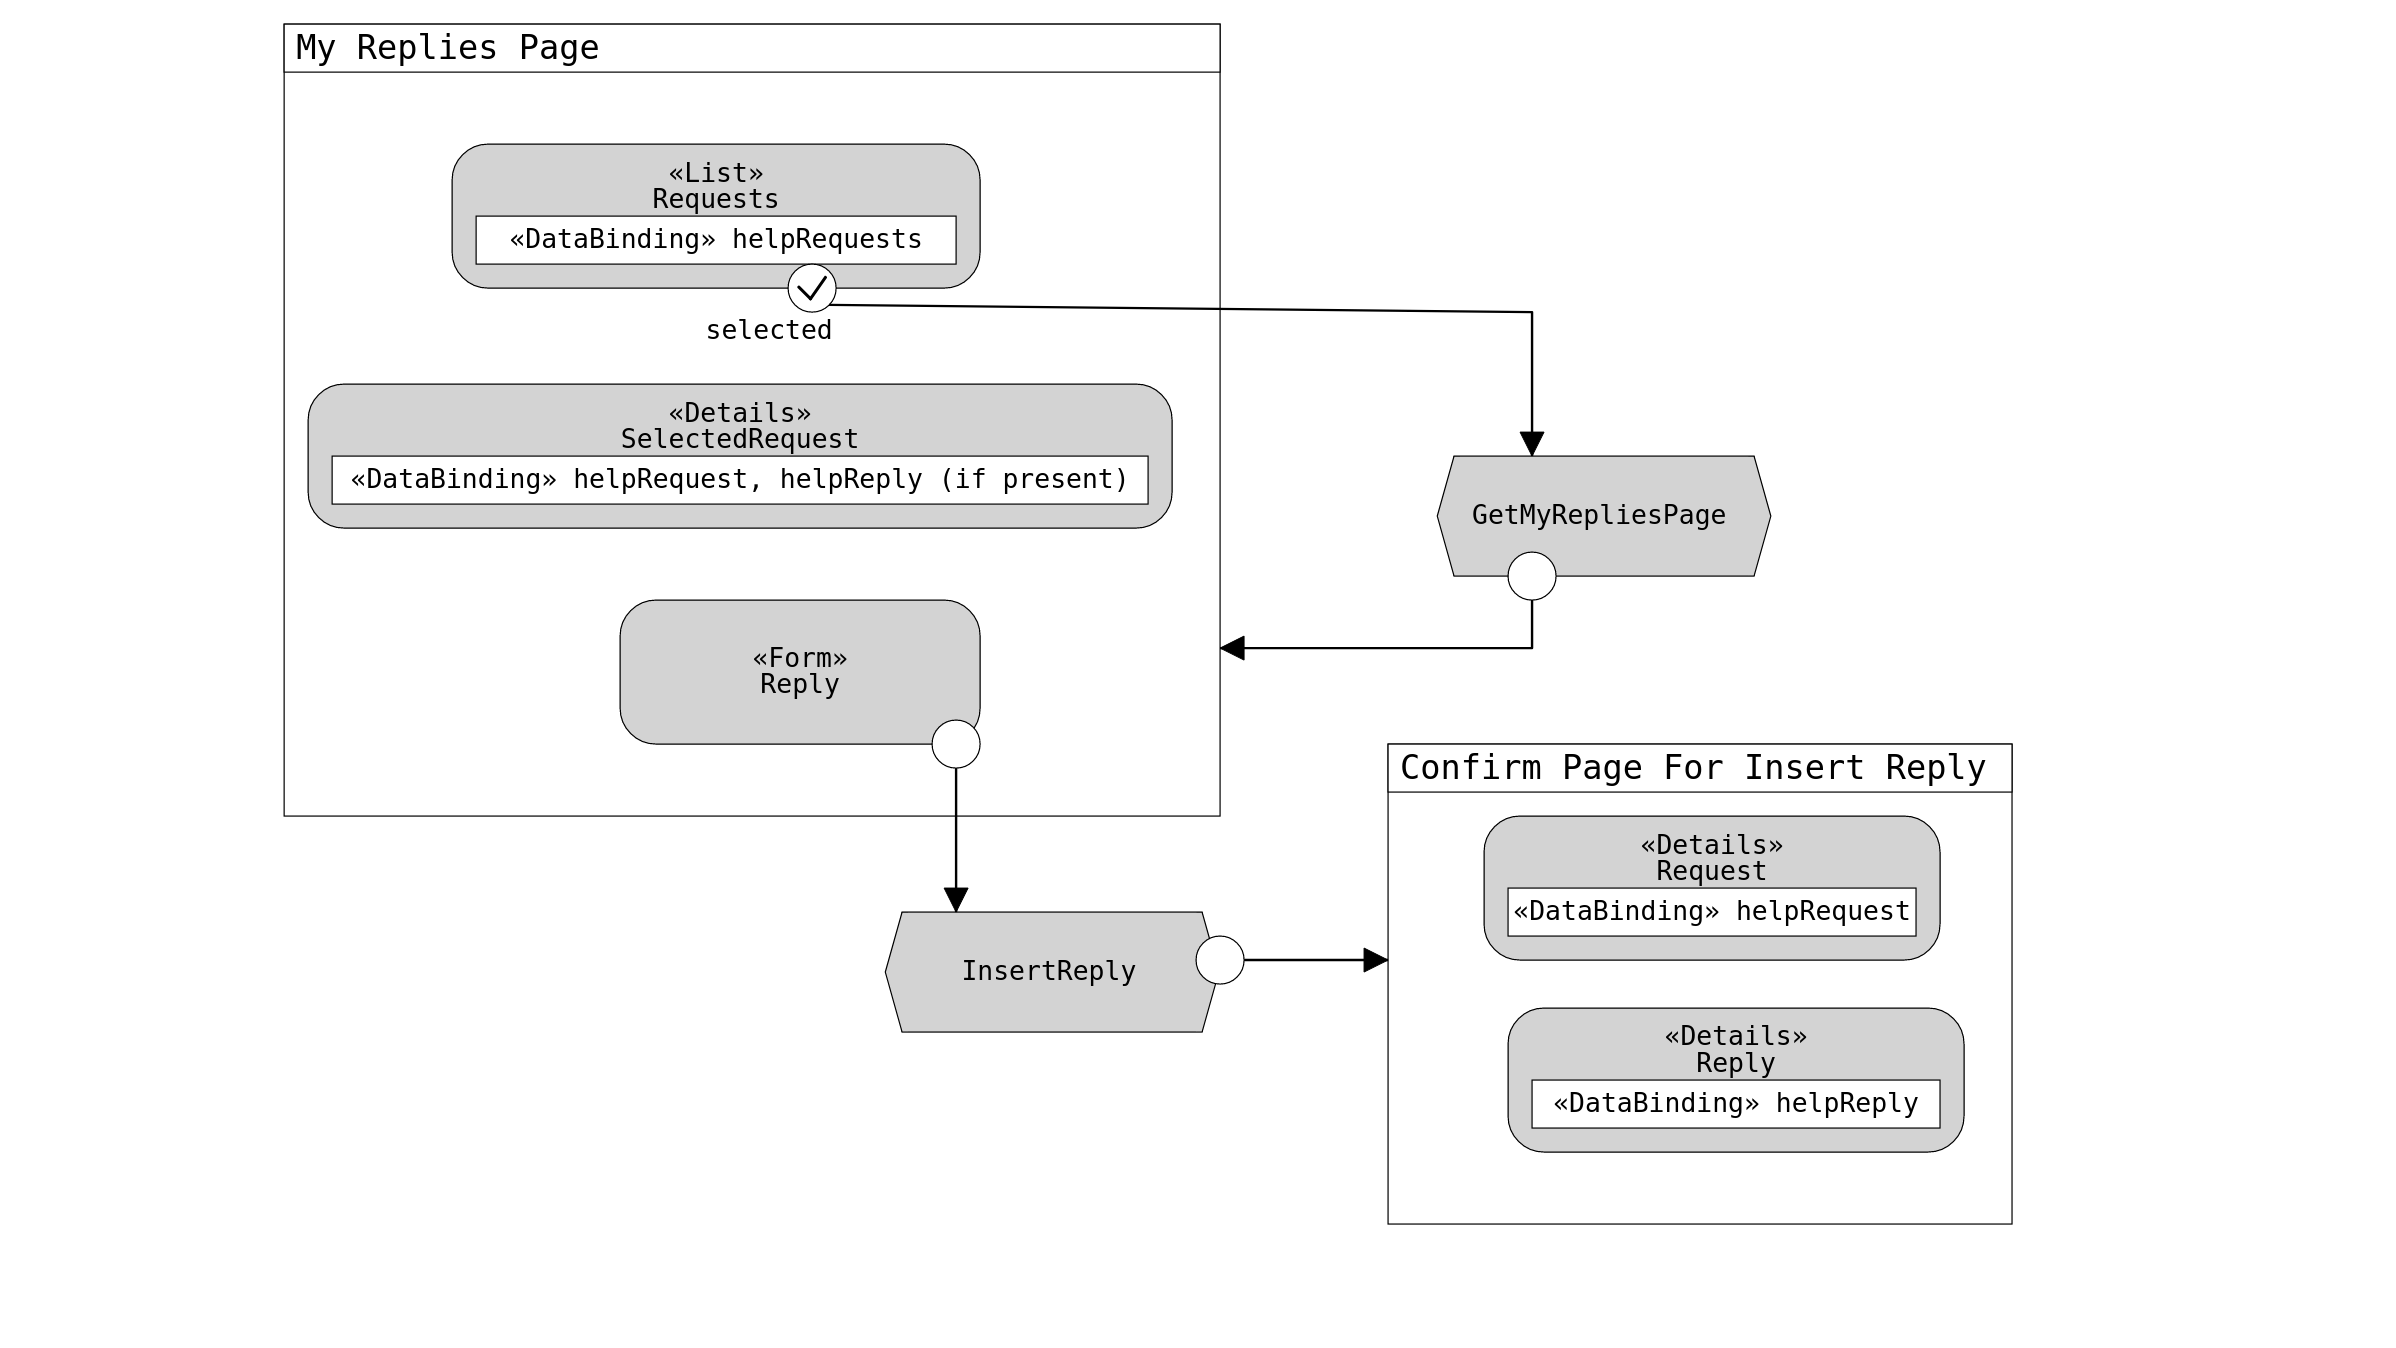
\includegraphics[scale=0.15]{diagrams/ui diagrams/farmer/my replies.png} 
    \caption{IFML diagram for the "My Replies" section of the farmer interface.}
\end{figure}
If the farmer is a best-performing farmer, in the main menu there is also a "My Replies" entry, that, if selected, brings to the My Replies Page. In this page, a list of the requests issued to the farmer is shown, ordered in descending temporal order. For each request, the asking farmer, the title and the date are shown. As in the My Requests section, only the last 20 requests are shown in the PC version of the website, while only the last 10 ones are displayed in the mobile version of the website, and a "Previous" and "Next" button are present to visualize other requests. Requests which have been already replied by the farmer are marked to distinguish them from unanswered ones, and requests that haven't been read yet by the farmer are highlighted. \newline
By selecting a request in the list, the farmer is shown in the My Replies Page also the text of the request, and if he/she has already replied to the request also the text of the response, together with the related feedback, if present.
If the farmer has not replied to the request, a form for inserting the reply is present. After submitting this form, the farmer is shown a confirmation page, with all details regarding the reply and the corresponding request, together with a confirmation message.\footnote{See \textit{RASD - 3.2.4 Use cases}, Use Case 23.} In the mobile version of the website, when selecting a request from the list in the My Replies Page, the request and the response (if present) are shown in another view, and also the form for inserting the request is shown in another dedicated view, accessible from the previous one.\newline
In the My Replies Page there is a "Back" button for going back to the Farmer Home Page, while in the Confirm Page For Insert Reply there is a "Back" button for going back to the My Replies Page.

\subsubsection{"Forum" section}
\begin{figure}[H]
    \centering
     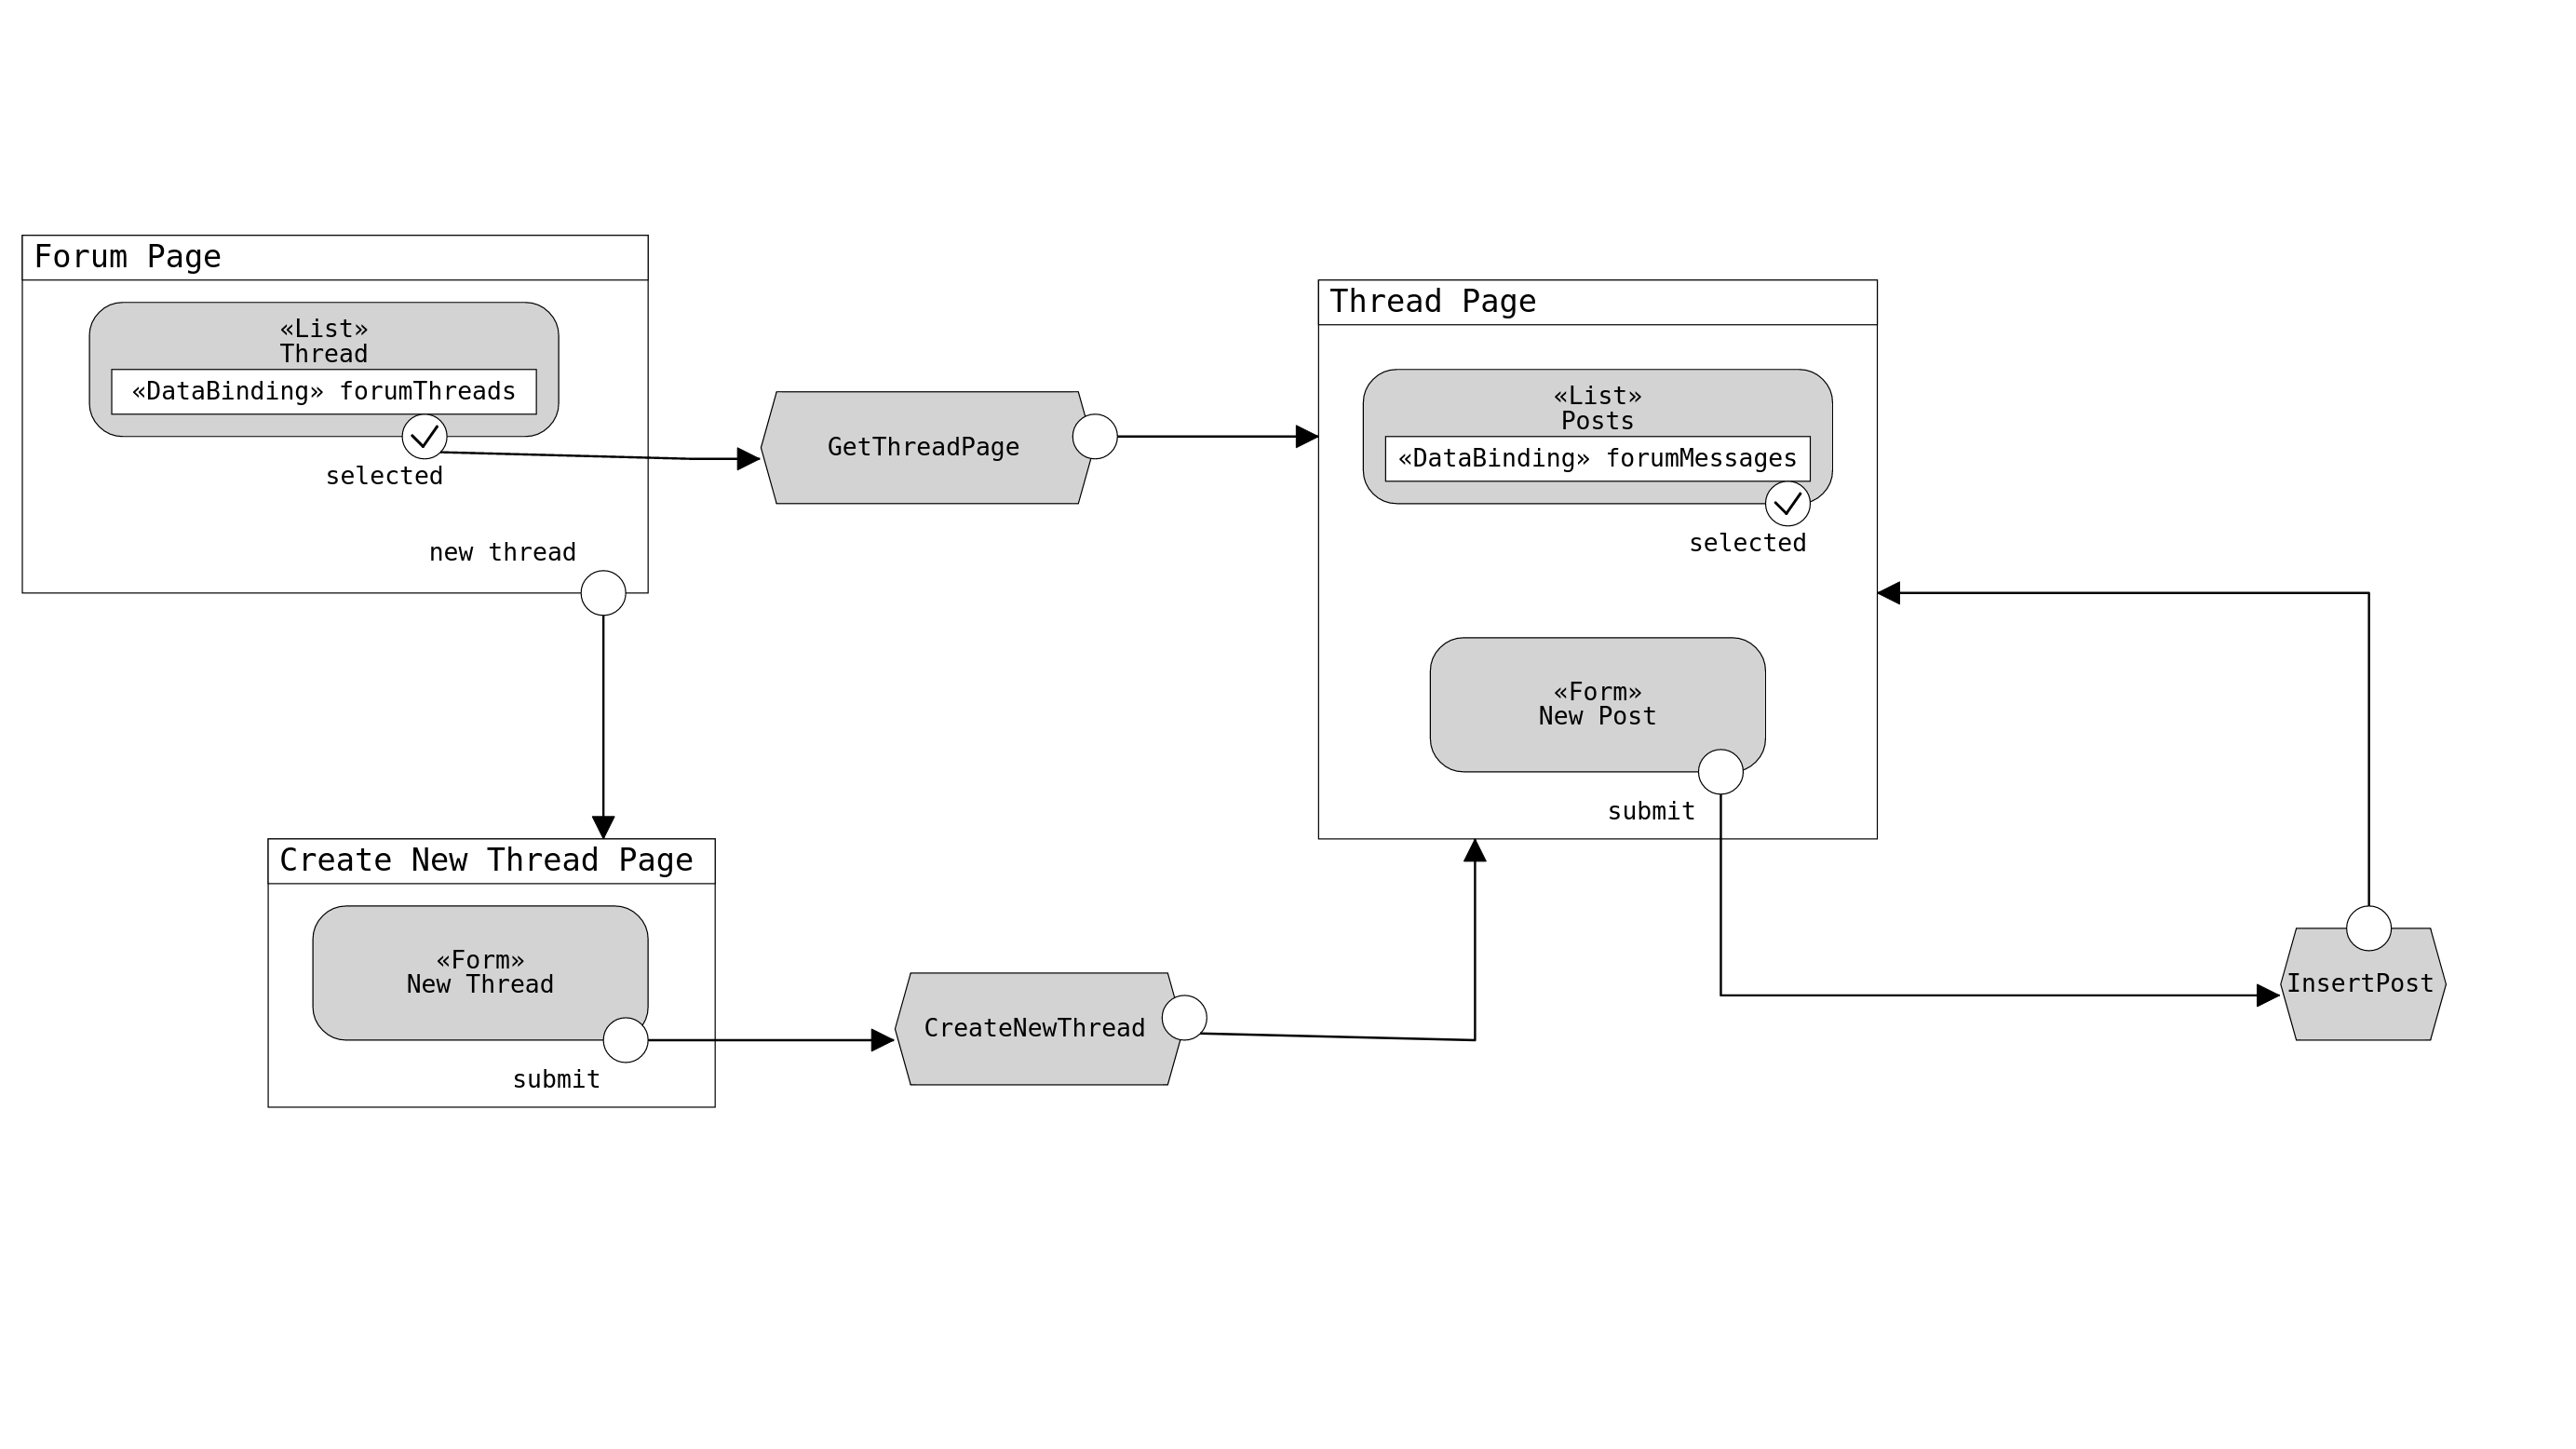
\includegraphics[scale=0.15]{diagrams/ui diagrams/farmer/forum.png} 
    \caption{IFML diagram for the "Forum" section of the farmer interface.}
\end{figure}
By selecting the "Forum" entry of the main menu, the user is displayed the Forum Page, which contains a list of the threads present in the forum ,together with a "New Thread" button. \newline
By selecting one of the threads in the Forum Page, the user accesses a Thread Page, which contains a list of the messages posted in the forum in descending temporal order, together with a form for inserting a new post. Only the last 20 messages posted are present - 10 in the mobile version of the website -, and there are a "Previous" and "Next" button for navigating between the groups of messages. When the user submits the form for posting a new message, the Thread Page is shown again, containing the new message in the list of the posted messages.\footnote{See \textit{RASD - 3.2.4 Use cases}, Use Case 26.} If the website is visited from a mobile device, the form for inserting a new message is displayed in a dedicated page.\newline
If the user selects the "New Thread" button in the Forum Page, a page with a form for creating a new thread is shown. When the user submits this form, he/she is shown the Thread Page for the new thread.\footnote{See \textit{RASD - 3.2.4 Use cases}, Use Case 25.} \newline
In the Forum Page there is a "Back" button for going back to the Farmer Home Page, while in the Thread Page and in the Create New Thread Page there is a "Back" button for going back to the Forum Page.

\subsection{Agronomist Interface}
The Home Page for agronomists contains a menu, from which the user can access the four sections of the interface: "Daily Plan", "Farms", "Weather Forecasts", "My Replies". \newline
If there are any notifications for the agronomist - e.g., a new request has been issued to him/her -, they are displayed in the Home Page.\newline
If it's the first time that the agronomist accesses the \verb|DREAM| system, a form for entering his personal and working data is present in the Home Page.\footnote{See \textit{RASD - 3.2.4 Use cases}, Use Case 2.}\newline
All pages represented in the diagram contain the main menu (not displayed in the diagram for the sake of simplicity), so that the user can freely navigate from one section to another without passing through the Home Page. 
\begin{center}
    \begin{sidewaysfigure}
    \includegraphics[scale=0.07]{diagrams/ui diagrams/agronomist/agronomist.png}
    \caption{IFML diagram for the agronomist portion of the interface.}
\end{sidewaysfigure}
\end{center}
\subsubsection{"Daily Plan" section}
\begin{figure}[H]
    \centering
     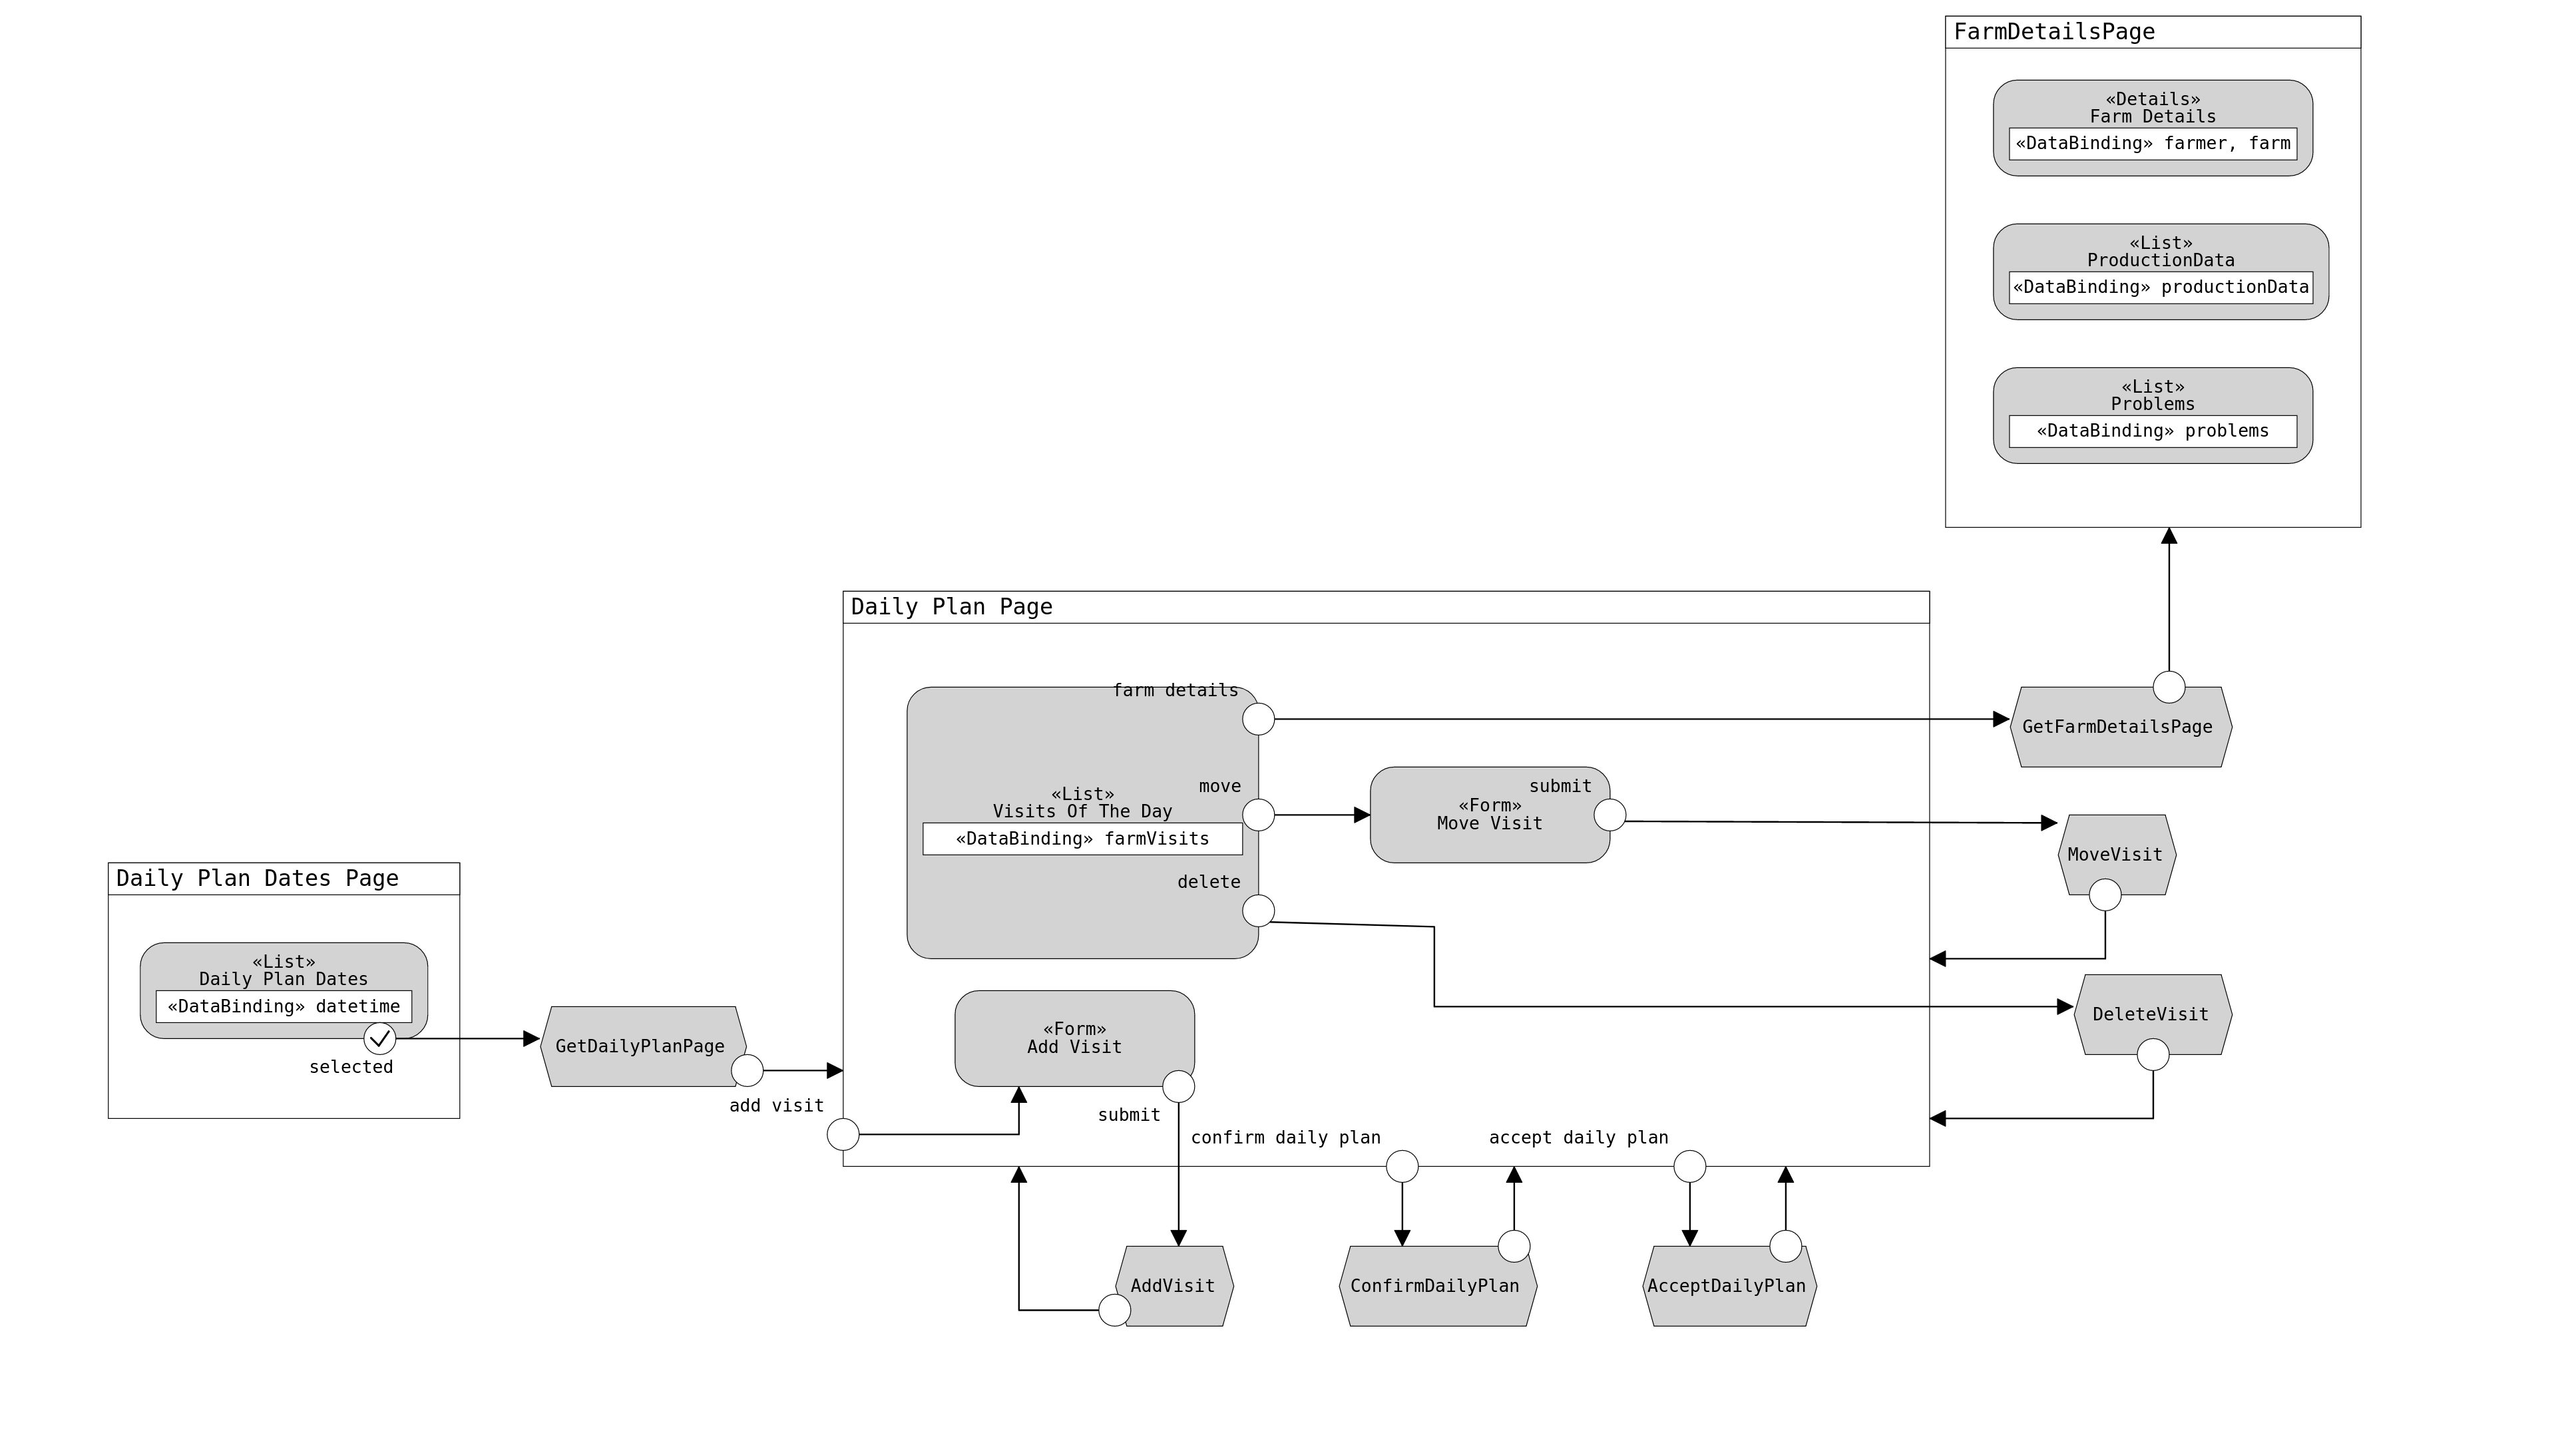
\includegraphics[scale=0.1]{diagrams/ui diagrams/agronomist/daily plan.png} 
    \caption{IFML diagram for the "Daily Plan" section of the agronomist interface.}
\end{figure}
By selecting the "Daily Plan" entry of the main menu, the user is shown the Daily Plan Dates Page, which displays a list of 7 working days, beginning from the current one.\newline
When the user selects one of these days, he/she accesses the Daily Plan Page, which displays the list of visits scheduled for the chosen day. \newline
If the daily plan has not been accepted yet, there are a "Farm Details", "Move" and "Delete" buttons for each visit, together with an "Add Visit" button and an "Accept Daily Plan" button. By clicking on a "Move" button related to a certain visit, the user is shown a form for selecting the new starting time for the visit, and after submitting this form, he/she is shown the daily plan with the visit moved to the desired starting time.\footnote{See \textit{RASD - 3.2.4 Use cases}, Use Case 9.} By clicking on the "Delete" button related to a certain visit, the user deletes the visit from the daily plan.\footnote{See \textit{RASD - 3.2.4 Use cases}, Use Case 10.} By clicking on the "Add Visit" button, the user is shown a form for adding a new visit to the daily plan, and when he/she submits this form, the visit is added to the daily plan.\footnote{See \textit{RASD - 3.2.4 Use cases}, Use Case 11.} If the user clicks on the "Accept Daily Plan" button, and if the \verb|DREAM| system allows this operation, the Daily Plan Page is shown to the user without the "Move", "Delete", "Add Visit" and "Accept Daily Plan" button, and with a confirmation message that the daily plan has been accepted. If the \verb|DREAM| does not allow the agronomist to accept the daily plan, the Daily Plan Page is shown again with the same visits and buttons as before clicking the "Accept Daily Plan" button, together with an error message.\footnote{See \textit{RASD - 3.2.4 Use cases}, Use Case 7.}\newline
If the daily plan has been accepted, and the last hour of the working day of a daily plan has passed, there are a "Farm Details", "Move" and "Delete" buttons for each visit, an input field for each visit for inserting a report, and an "Add Visit" button and a "Confirm Daily Plan" button. The "Move", "Delete" and "Add Visit" buttons are exactly the same as when the daily plan has not been accepted yet. When the user selects the "Confirm Daily Plan" button, the Daily Plan Page is shown to the user without the "Move", "Delete", "Add Visit" and "Accept Daily Plan" button, and with a confirmation message that the daily plan has been confirmed.\footnote{See \textit{RASD - 3.2.4 Use cases}, Use Case 12.} \newline
If the user selects the "Farm Details" button related to a certain farm, the Farm Details Page of the selected farm is shown. It contains some details about the farm and the farmer who owns the farm - location of the farm, name and surname of the farmer - and the list of production data and problems inserted by the farmer since the last visit of the agronomist to the farm.\footnote{See \textit{RASD - 3.2.4 Use cases}, Use Case 8.}\newline
A "Back" button in the Daily Plan Dates Page brings back to the Agronomist Home Page, a "Back" button in the Daily Plan page brings back to the Daily Plan Dates Page, and a "Back" button in the Farm Details Page brings back to the Daily Plan Page.

\subsubsection{"Farms" section}
\begin{figure}[H]
    \centering
     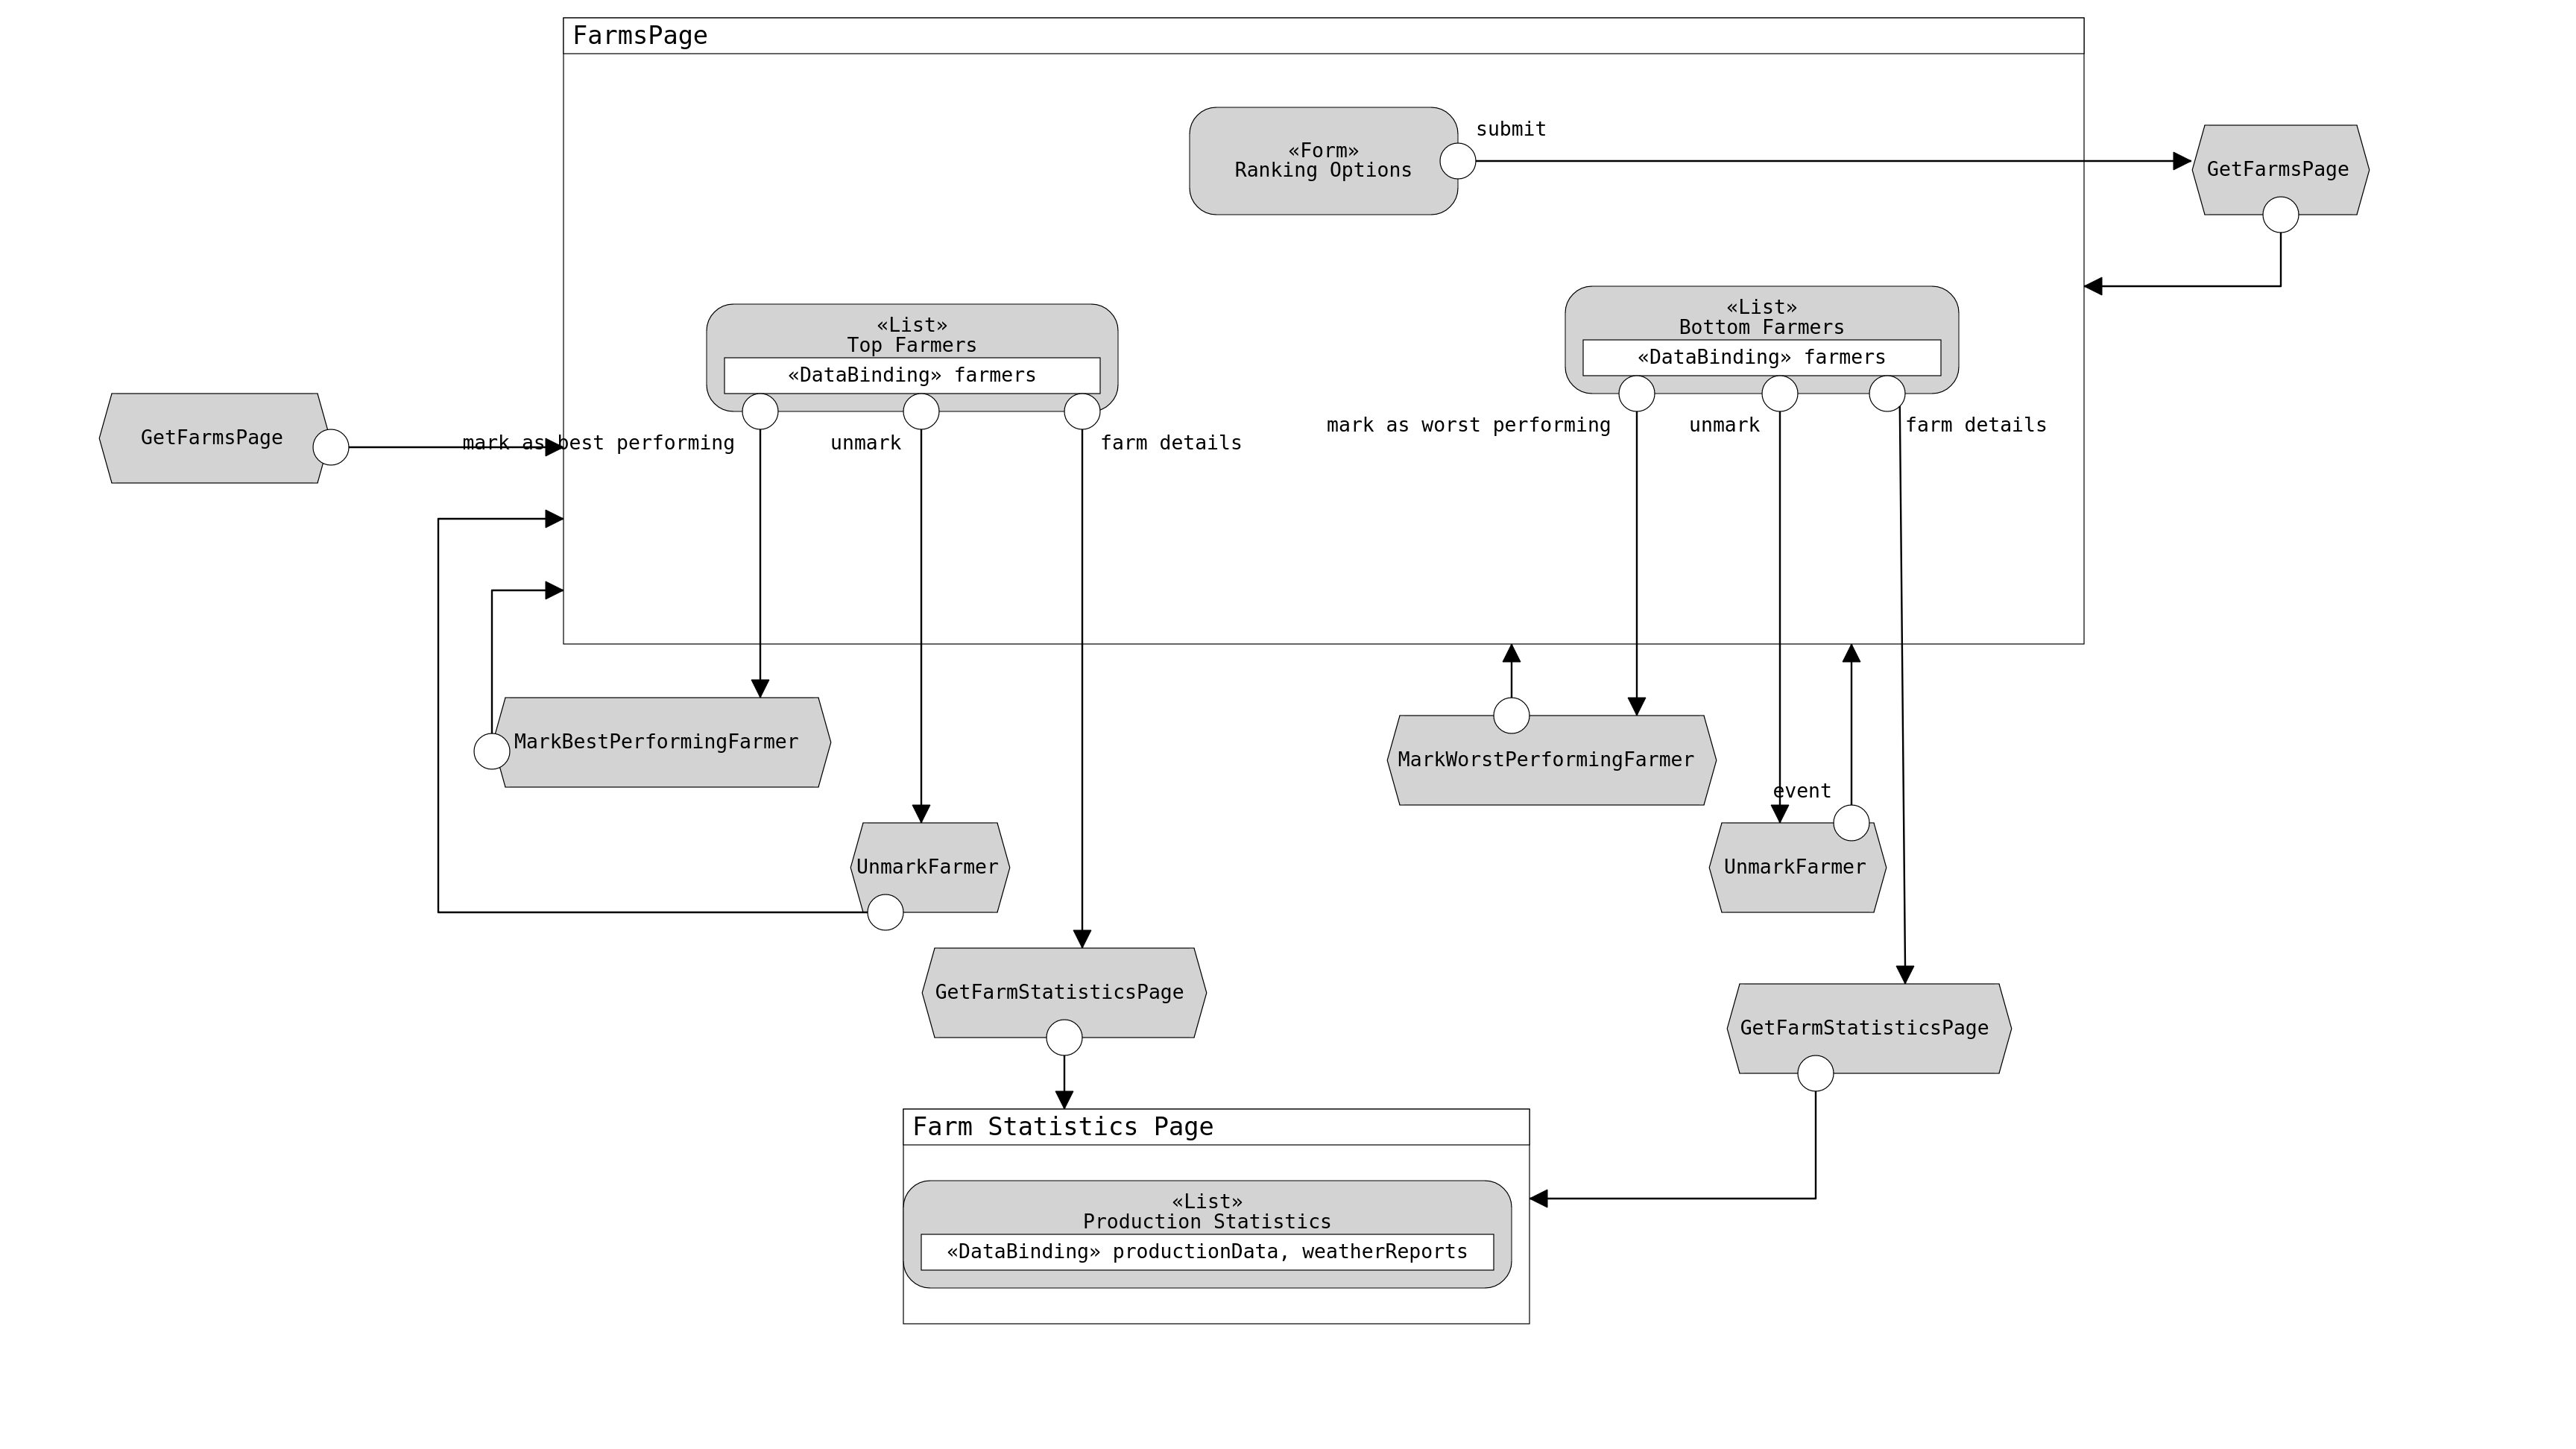
\includegraphics[scale=0.1]{diagrams/ui diagrams/agronomist/farms.png} 
    \caption{IFML diagram for the "Farms" section of the agronomist interface.}
\end{figure}
By selecting the "Farms" entry of the main menu, the user is shown the Farms Page, which contains a form that allows the agronomist to select some options for ranking the farmers in the area he/she is assigned to. When the user submits this form, the Farms Page displays a list of the best farmers according to the criteria chosen by the agronomist, and a list of the worst farmers according to the same criteria.\footnote{See \textit{RASD - 3.2.4 Use cases}, Use Case 15.} For each farmer there is a "Farm Details" button, which brings to a Farm Statistics Page, where monthly data about the farm production are shown. For each farmer in the first list, if not already marked as best- or worst-performing, there is a "Mark as best-performing" button\footnote{See \textit{RASD - 3.2.4 Use cases}, Use Case 16.}; for each farmer in the second list, if not already marked as best- or worst-performing, there is a "Mark as worst-performing" button. For each best- or worst-performing farmer there is an "Unmark" button\footnote{See \textit{RASD - 3.2.4 Use cases}, Use Case 17.}. \newline
A "Back" button in the Farms Page allows the user to go back to the Agronomist Home Page, while a "Back" button in the Farm Statistics Page allows the user to go back to the Farms Page.

\subsubsection{"Weather Forecasts" section}
This section of the website is analogous to the farmers' "Weather Forecasts" section, therefore the reader is redirected to section 3.2.2 of this document. The only difference between the agronomists' and farmers' Weather Forecasts Page is that the form in the agronomists' page allows the user to select not only the date, but also the location (in the area where the agronomist works) to consider for the forecasts.

\subsubsection{"My Replies" section}
This section of the website is analogous to the farmers' "My Replies" section, therefore the reader is redirected to section 3.2.5 of this document.

\subsection{Policy Maker Interface}
The Home Page for policy makers contains a menu, from which the user can access the two sections of the interface: "Farms" and "Initiatives Analysis".
All pages represented in the diagram contain the main menu (not displayed in the diagram for the sake of simplicity), so that the user can freely navigate from one section to another without passing through the Home Page. 
\begin{center}
    \begin{sidewaysfigure}
    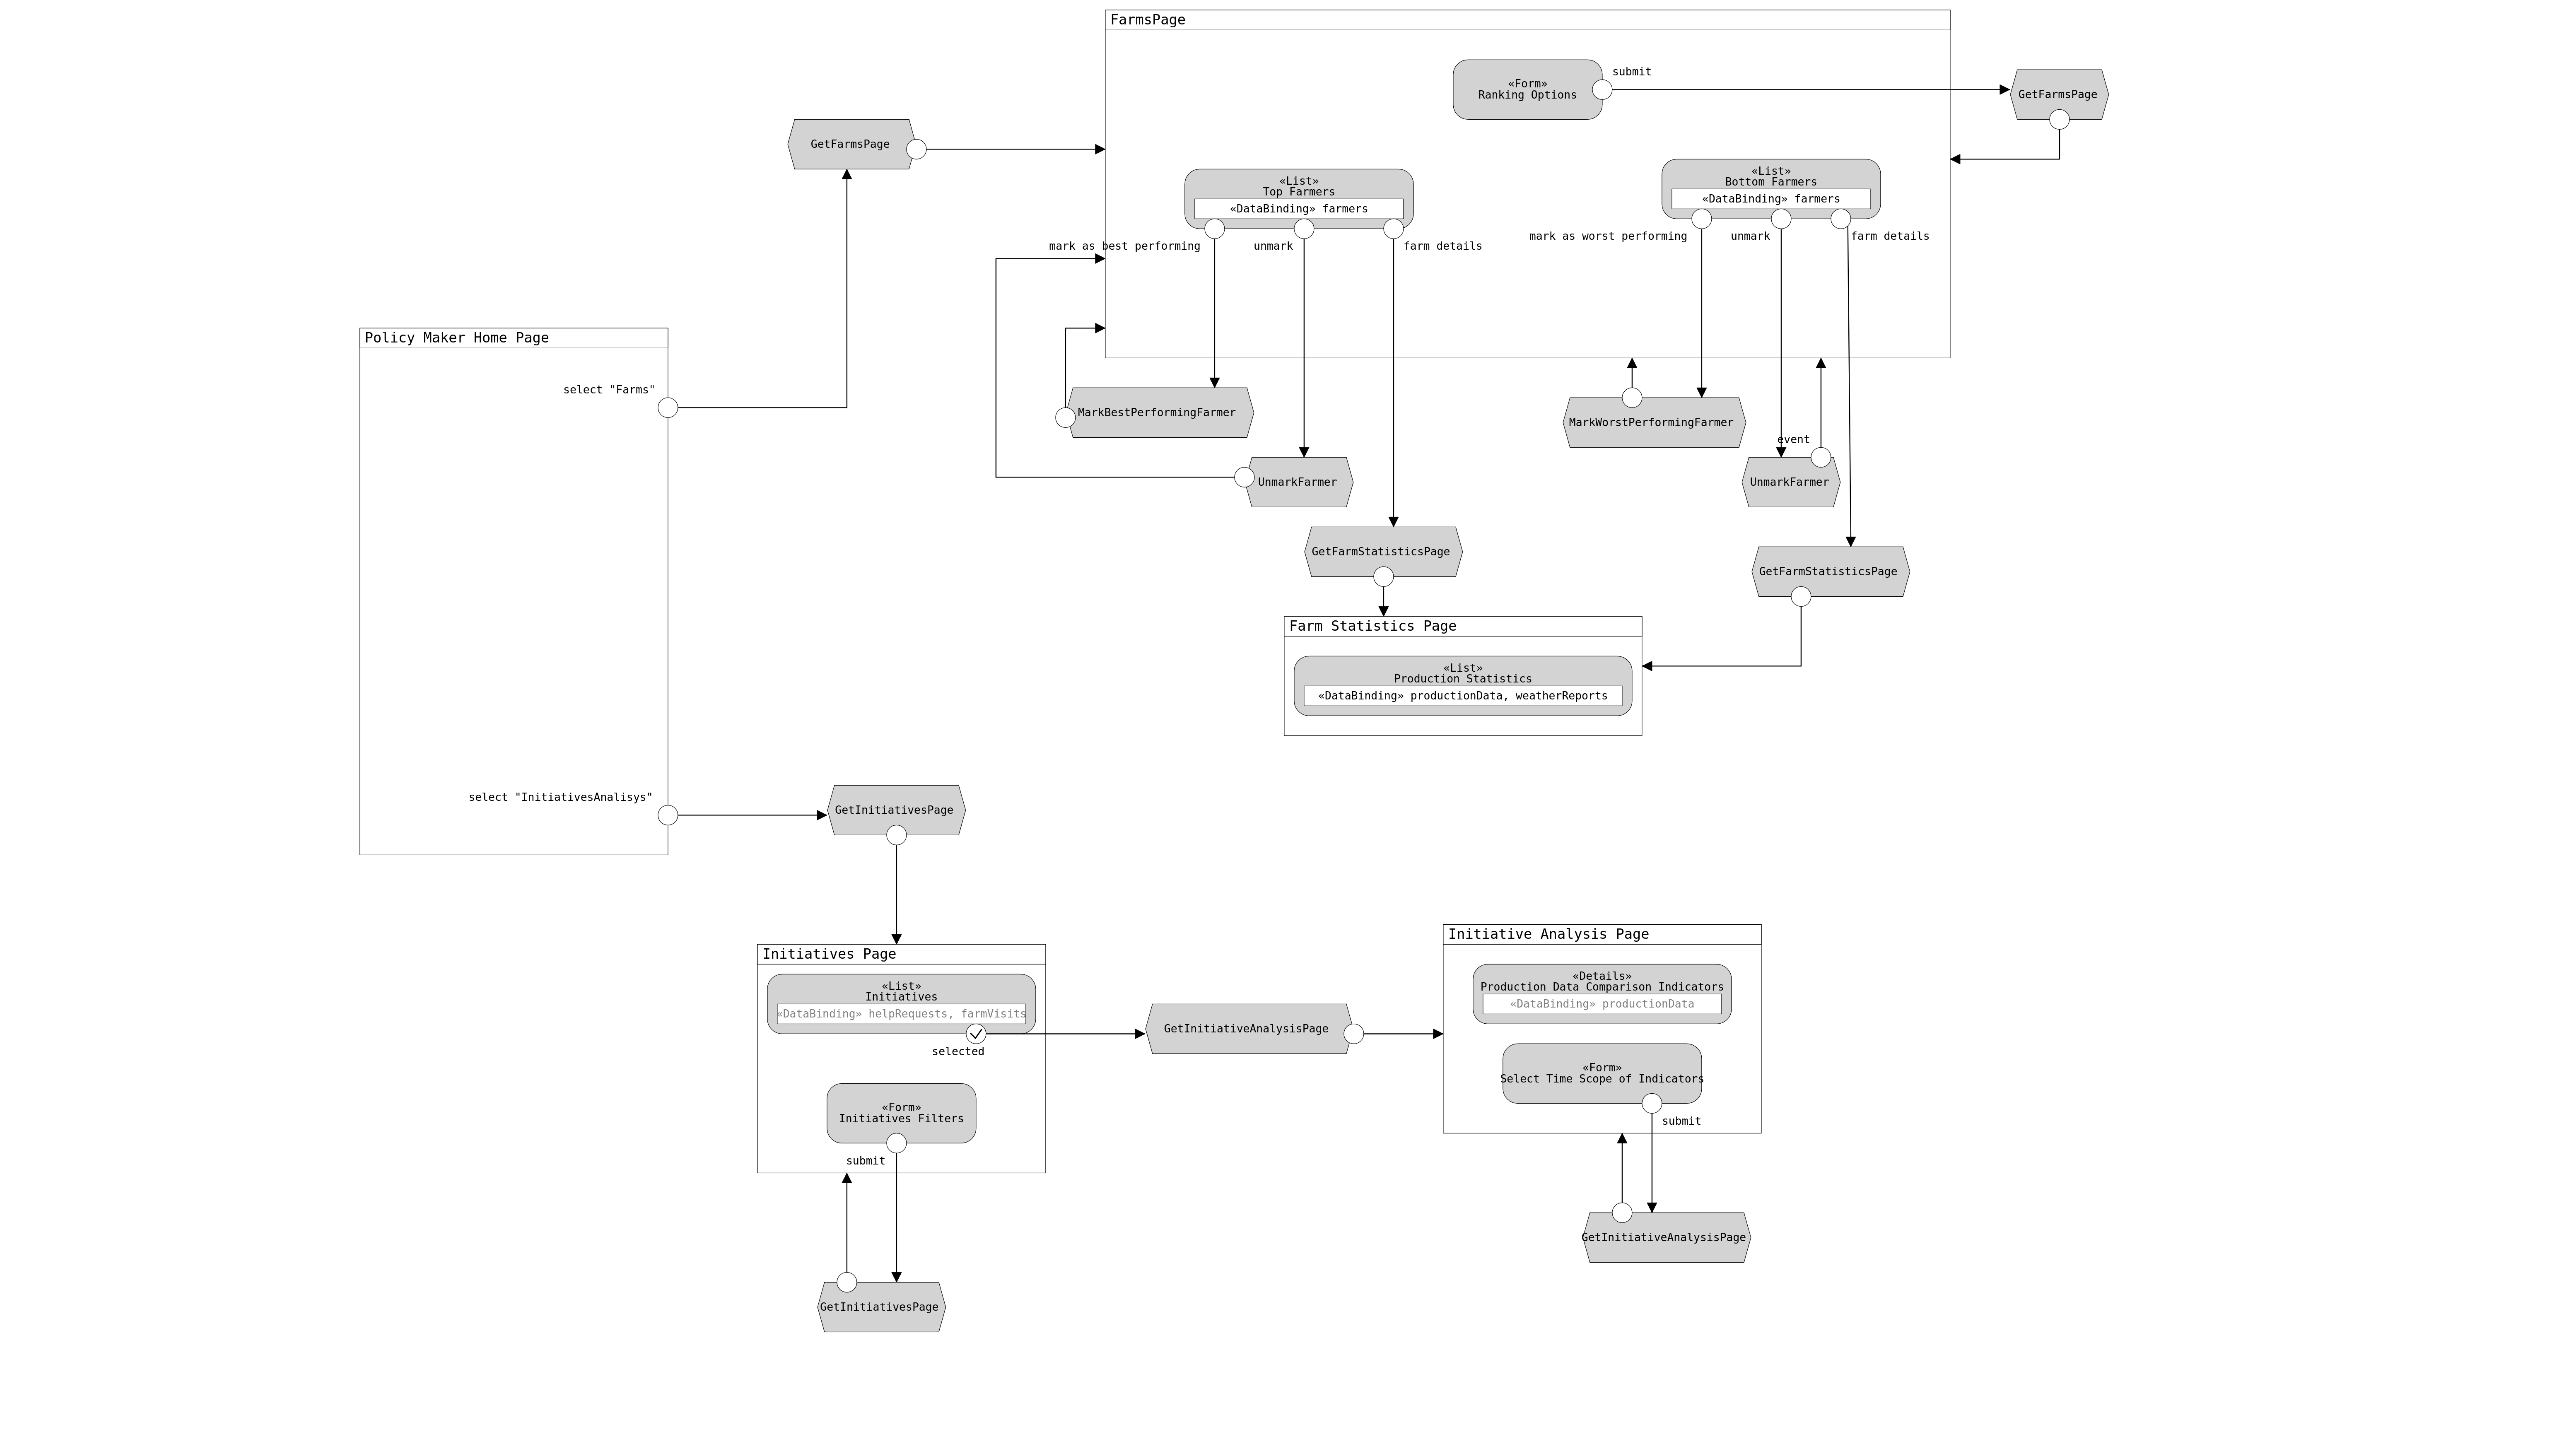
\includegraphics[scale=0.11]{diagrams/ui diagrams/policymaker/policymaker.png}
    \caption{IFML diagram for the policy maker portion of the interface.}
\end{sidewaysfigure}
\end{center}
\newpage

\subsubsection{"Farms" section}
This section of the website is analogous to the agronomist' "Farms" section, therefore the reader is redirected to section 3.3.2 of this document.
The only difference is that policy makers can visualize farms located in all the Telangana state, while agronomists can visualize only the ones belonging to the area they are assigned to.

\subsubsection{"Initiatives Analysis" section}
\begin{figure}[H]
    \centering
     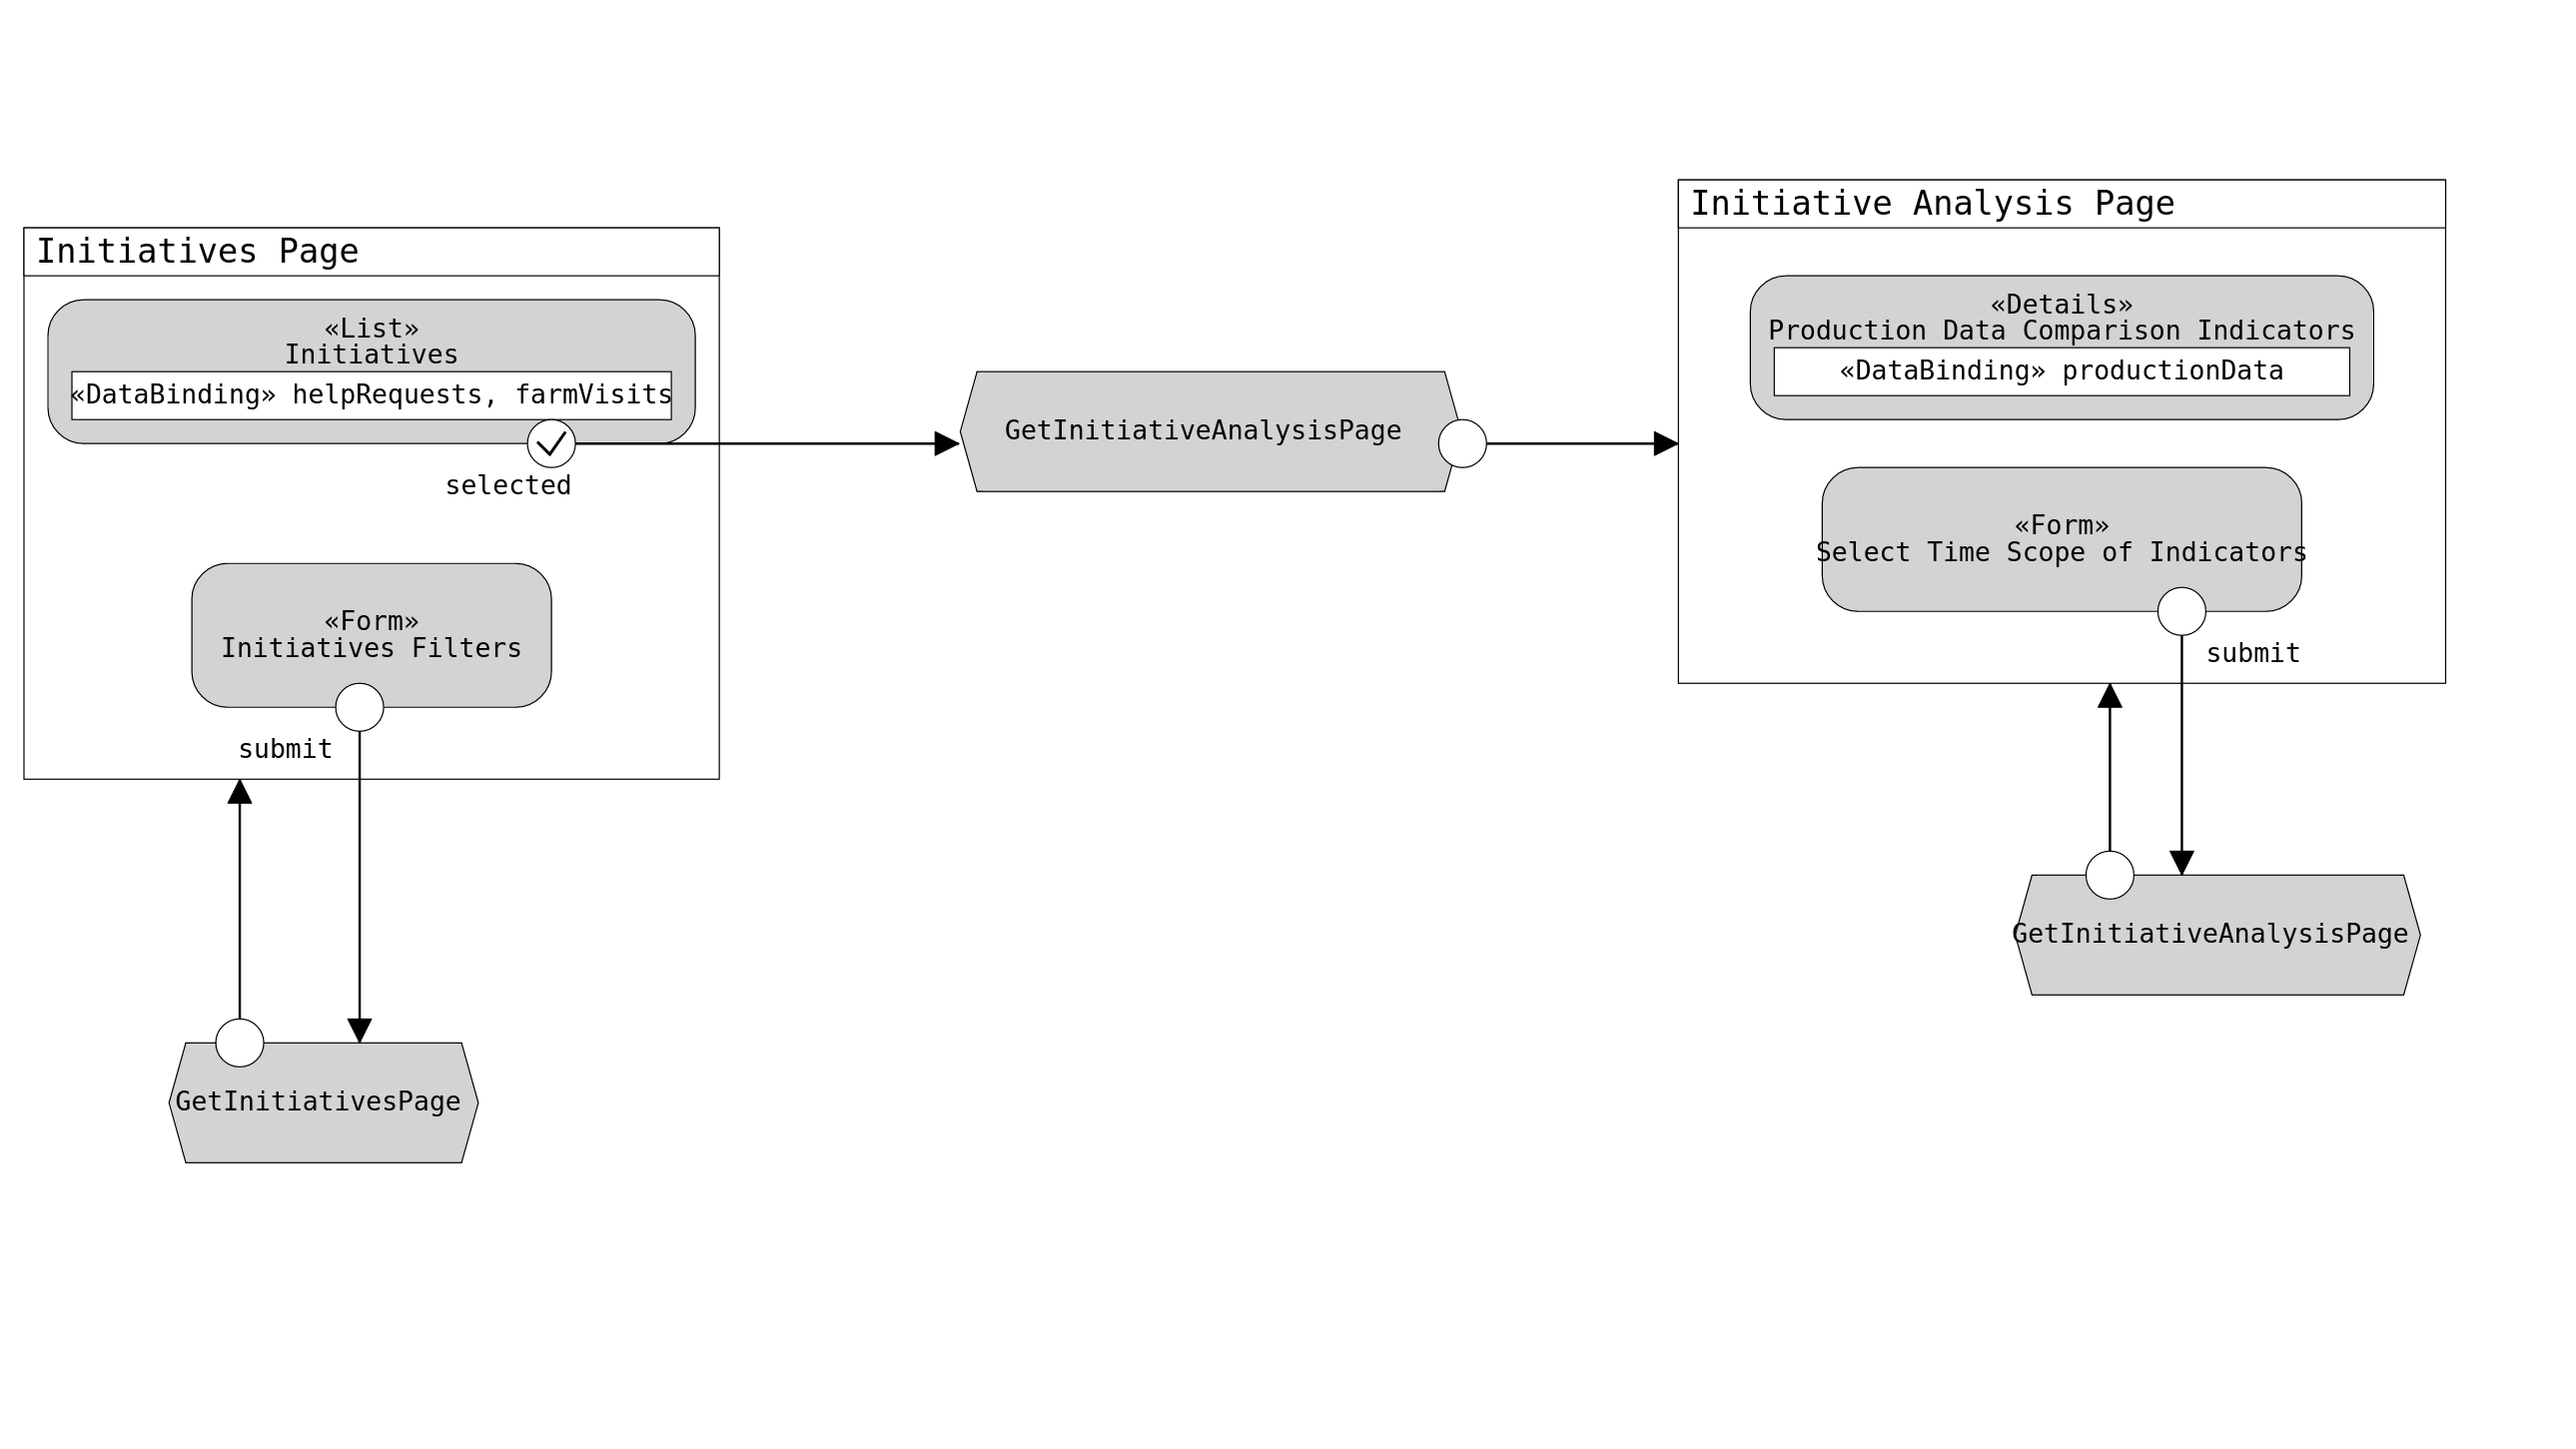
\includegraphics[scale=0.17]{diagrams/ui diagrams/policymaker/initiatives analysis.png} 
    \caption{IFML diagram for the "Initiatives Analysis" section of the policy maker interface.}
\end{figure}
By selecting the "Initiatives Analysis" entry in the main menu, the user is shown the Initiatives Page, which contains the list of initiatives recorded into the \verb|DREAM| system, ordered in descending temporal order. Only the last 50 initiatives are displayed, and two buttons "Next" and "Previous" allow the user to navigate through other sets of initiatives. In the page there is also a form that allows the user to filter the initiatives according to the type, date, area, etc.. \newline
By selecting an initiative in the list, the user is shown the corresponding Initiative Analysis Page, where some indicators comparing the farm production one month before and one month after the initiative are displayed, together with a form that allows to user to change the time scope of these indicators.\footnote{See \textit{RASD - 3.2.4 Use cases}, Use Case 18.} \newline
A "Back" button in the Initiatives Page brings to the Policy Maker Home Page, while a "Back" button in the Initiatives Analysis Page brings to the Initiatives Page.

\newpage
\section{Requirements Traceability}
This section shows the mapping between the requirements listed in \textit{RASD - 3.2.1 Use cases} and the components presented in the section  2.2 of this document.
\newline
\newline
The following table shows how business logic components presented in the section  2.2 of this document implement the requirements of the \verb|DREAM| system.
\rowcolors{2}{gray!15}{gray!35}
\begin{longtable}[c]{|m{0.15cm}|m{0.15cm}|m{0.15cm}|m{0.15cm}|m{0.15cm}|m{0.15cm}|m{0.15cm}|m{0.15cm}|m{0.15cm}|m{0.15cm}|}
 \caption{Traceability matrix of components to requirements.}
 \label{comp-req mapping}
%%%%%%%%%%%%%%%%%%%%%%%%%%%%%%%%%%
 \hline
 \multicolumn{10}{|c|}{\cellcolor{white}Mapping between Components and Requirements}
 % do not write anything here
 \endfirsthead
 \hline
  \cellcolor{yellow!30} & \cellcolor{white}FS & \cellcolor{white}DPS & \cellcolor{white}AS & \cellcolor{white}SS & \cellcolor{white}WS & \cellcolor{white}PDS & \cellcolor{white}RS & \cellcolor{white}HRS &  \cellcolor{white}AUTHS \\
 \endhead
 % do not write anything here
 \endfoot
 % do not write anything here
 \endlastfoot
%%%%%%%%%%%%%%%%%%%%%%%%%%%%%%%%%
 \hline
  \cellcolor{yellow!30} & \cellcolor{white}FS & \cellcolor{white}DPS & \cellcolor{white}AS & \cellcolor{white}SS & \cellcolor{white}WS & \cellcolor{white}PDS & \cellcolor{white}RS & \cellcolor{white}HRS &  \cellcolor{white}AUTHS \\
 \hline
 R1 &   &  &  &  X &  &   &  &   &    \\
 \hline
 R2 &  &  &  &   &  &   &  &   &     \\
 \hline
 R3 &  &  &  &   &  &   &  &   &     \\
 \hline
 R4 &  &  &  &  &  &   &  &   &     \\
 \hline
 R5 &  &   &   &   &   &   &  &   &     \\
 \hline
 R6 &  &   &   &   &   &   &   &   &      \\
 \hline
 R7 &  &   &   &   &   &   &   &   &      \\
 \hline
 R8 &  &   &   &   &   &   &   &   &     \\
 \hline
 R9 &   &  &   &   &   &   &   &   &      \\
 \hline
 R10 &   &  &  &   &   &   &   &   &     \\
 \hline
 R11 &   &  &  &   &   &   &   &   &      \\
 \hline
 R12 &    &   &  &   &   &   &   &   &   \\
 \hline
 R13 &    &   &  &   &   &   &   &   &   \\
 \hline
 R14 &    &   &  &   &   &   &   &   &   \\
 \hline
 R15 &   &  &   &   &   &   &   &   &      \\
 \hline
 R16 &   &  &   &   &   &   &   &   &      \\
 \hline
 R17 &   &   &  &   &  &   &   &   &      \\
 \hline
 R18 &   &   &  &   &   &   &   &   &      \\
 \hline
 R19 &   &   &   &  &   &   &   &   &      \\
 \hline
 R20 &   &   &   &  &  &   &   &   &     \\
 \hline
 R21 &   &   &   &  &   &   &   &   &     \\
 \hline
 R22 &   &   &   &   &   &   &  &   &     \\
 \hline
 R23 &   &   &   &   &   &   &   &   &     \\
 \hline
 R24 &   &   &   &   &   &   &   &   &     \\
 \hline
 R25 &   &   &   &   &   &   &   &   &     \\
 \hline
 R26 &   &   &   &   &  &   &   &   &      \\
 \hline
 R27 &   &   &   &   &  &   &   &   &      \\
 \hline
 R28 &   &   &   &   &   &  &   &   &      \\
 \hline
 R29 &   &   &   &   &   &  &   &   &  \\
 \hline
 R30 &   &   &   &   &   &  &   &   &      \\
 \hline
 R31 &   &   &   &   &   &  &   &   &      \\
 \hline
 R32 &   &   &   &   &   &  &   &   &      \\
 \hline
 R33 &   &   &   &   &   &  &   &   &      \\
 \hline
 R34 &   &   &   &   &   &   &   &  &      \\
 \hline
 R35 &   &   &   &   &   &   &   &  &      \\
 \hline
 R36 &   &   &   &   &   &   &   &  &      \\
 \hline
 R37 &   &   &   &   &   &   &   &  &      \\
 \hline
 R38 &   &   &   &   &   &   &  &   &     \\
 \hline
 R39 &   &   &   &   &   &   &  &   &     \\
 \hline
 R40 &   &   &   &   &   &   &  &   &     \\
 \hline
 R41 &   &   &   &   &   &   &  &   &      \\
 \hline
 R42 &   &   &   &   &   &   &  &   &      \\
 \hline
 R43 &   &   &   &   &   &   &  &   &      \\
 \hline
 R44 &   &   &   &   &   &   &  &   &      \\
 \hline
 R45 &   &   &   &   &   &   &  &   &      \\
 \hline
 R46 &   &   &   &   &   &   &  &   &      \\
 \hline
 R47 &   &   &   &   &   &   &  &   &      \\
 \hline
\end{longtable}

Legend:
\begin{itemize}
    \item FS: ForumService
    \item DPS:DailyPlanService
    \item AS: AnalyticsService
    \item SS: SensorService
    \item WS: WeatherService
    \item PDS:ProductionDataService
    \item RS: RankingService
    \item HRS: HelpRequestService
    \item AUTHS: AuthenticationService
\end{itemize}

Here a brief explanation of the mapping presented in the previous table is provided.

\begin{itemize}
    \item R1 - \verb|DREAM| collects soil moisture data from the soil moisture sensors: SensorService
\end{itemize}

\newpage
\section{Implementation, integration and test plan}
\subsection{Implementation and integration}
\setlength{\parskip}{.5em}
As outlined in the component diagram, there is a fairly small number of dependencies between components; this is due to the fact DREAM is made up of many independent features.

\par The first part of the system to bring up is the \textbf{DBMS} along with the \textbf{Database Abstraction Layer}, since basically every other component relies on database access to store and retrieve data. The DBAL component will not be implemented in-house; instead, a robust pre-existing solution provided by the adopted framework will be used.

\par The first component that must be set up is the \textbf{AuthenticationService}, since authentication is required for all other components to function. Again, this being a generic feature, it will be provided by the framework and will only need to be configured for our use case.

\par Subsequently, work on the other backend components can begin and be carried on in parallel, with the exception of the \textbf{RankingService} which requires the development of other services to be complete (namely, the \verb|Weather| and \verb|ProductionData| components). Simultaneously with the development of each component, the required integrations will be performed. As already mentioned, components are loosely coupled, thus a more detailed integration plan would be redundant.

\par As for frontend development, thanks to the specific architecture chosen, it is possible to proceed with development of the web interface immediately after the completion of each component. This is preferable to developing the frontend strictly after the entire backend is ready, as it allows for immediate feedback on the specific feature being developed.

\subsection{Testing}
Due to the number of independent features in the system, it is crucial that \textbf{each component undergoes unit testing}. Testing will begin as soon as the development of each component is complete, and will focus mostly on the business logic, and to a lesser extent to presentation logic.

\par For our specific use case, integration testing is of minor significance, but still required for some specific cases (e.g. the \verb|RankingService| as explained above).

\par After the implementation and integration phase is complete and the system is deemed to be in a production-ready state, \textbf{stress testing} is also required due to the large number of users that will access the system simultaneously. This will be carried forward using specialized external services that allow sending a large number of requests while simulating real user behaviour.
\newpage
\section{Effort spent}
\newpage
\section{References}
\end{document}

